\documentclass[
11pt,%
tightenlines,%
twoside,%
onecolumn,%
nobibnotes,%
nofootinbib,%
superscriptaddress,%
noshowpacs,%
centertags]%
{revtex4-2}
\usepackage{ljm}
\setcaptionwidth{0.93\textwidth}

% --- ГРАФИКА (WINDOWS) ---
\usepackage{epstopdf} % Критично для Windows: конвертирует EPS на лету
\graphicspath{{figures/}} 

% --- СТИЛЬ ЖУРНАЛА ---
\usepackage{ljm} % Файл должен лежать рядом!

% --- МАТЕМАТИКА И ТАБЛИЦЫ ---
\usepackage{mathtools}
\usepackage{colortbl}
\usepackage{algorithm2e}
% \usepackage{multirow}
\usepackage{makecell}  %new line in one table cell

% --- TIKZ (ВНИМАНИЕ: Для журнала в итоге нужны EPS файлы) ---
\usepackage{pgf}
\usepackage{tikz}
\usepackage{nicematrix}
\usetikzlibrary{arrows, automata, fit, calc, positioning}

% --- ДОПОЛНИТЕЛЬНО ---
% \usepackage{soul}
\usepackage[makeroom]{cancel}
\newcommand{\mycomment}[1]{}

\usepackage[caption=false]{subfig}
\usepackage{wrapfig}

\begin{document}
%
\title{GLL-based Context-Free Path Querying for Neo4j}

% --- АВТОРЫ (Формат RevTeX) ---

\author{Vadim Abzalov}
\email[E-mail: ]{vadim.i.abzalov@gmail.com}
\affiliation{Saint Petersburg State University, St. Petersburg, Russia}

\author{Vlada Pogozhelskaya}
\email[E-mail: ]{vvpogozhelskaia@edu.hse.ru}
\affiliation{National Research University Higher School of Economics, St. Petersburg, Russia}

\author{Vladimir Kutuev}
\email[E-mail: ]{v.kutuev@spbu.ru}
\affiliation{Saint Petersburg State University, St. Petersburg, Russia}

\author{Olga Bachishche}
\email[E-mail: ]{bachisheo@gmail.com}
\affiliation{ITMO University, St. Petersburg, Russia}

\author{Semyon Grigorev}
\email[E-mail: ]{s.v.grigoriev@spbu.ru}
\affiliation{Saint Petersburg State University, St. Petersburg, Russia}


% --- АННОТАЦИЯ (Должна быть ДО maketitle) ---
\begin{abstract}
We propose a GLL-based \textit{context-free path querying} algorithm that handles queries in Extended Backus-Naur Form (EBNF) using Recursive State Machines (RSM). Utilization of EBNF allows one to combine traditional regular expressions and mutually recursive patterns in constraints natively. The proposed algorithm solves both the \textit{reachability-only} and the \textit{all-paths} problems for the \textit{all-pairs} and the \textit{multiple sources} cases. The evaluation on real-world graphs demonstrates that the utilization of RSMs increases the performance of query evaluation. Being implemented as a stored procedure for Neo4j, our solution demonstrates better performance than a similar solution for RedisGraph. The performance of our solution on regular path queries is comparable to the performance of the native Neo4j solution, and in some cases, our solution requires significantly less memory.
\end{abstract}

% --- КЛЮЧЕВЫЕ СЛОВА ---
\keywords{Graph database, graph querying, context-free path querying, CFPQ, reachability problem, all-paths problem, generalized LL, GLL}

% --- ГЕНЕРАЦИЯ ЗАГОЛОВКА ---
\maketitle
\renewcommand{\figurename}{Fig.} 
% --- MAIN CONTENT ---
\section{Introduction}

Context-free path querying (CFPQ) allows one to use context-free grammars to specify constraints on paths in edge-labeled graphs. Compared to regular path queries (RPQ), CFPQ is strictly more expressive: for instance, a context-free grammar can be built to find siblings or same-generation categories in a taxonomy~\cite{Azimov:2018:CPQ:3210259.3210264,Kuijpers:2019:ESC:3335783.3335791}. This expressiveness allows CFPQ to be used for graph analysis in such areas as bioinformatics (hierarchy analysis~\cite{zhangCfPgRdf}, similarity queries~\cite{SubgraphQueriesbyContextfreeGrammars}), data provenance analysis~\cite{8731467}, static code analysis~\cite{Zheng,10.1145/373243.360208}. Although a lot of algorithms for CFPQ have been proposed, poor performance on real-world graphs and bad integration with real-world graph databases and graph analysis systems are still problems that hinder the adoption of CFPQ.

The problem with the performance of the CFPQ algorithms in real-world scenarios was pointed out by Jochem Kuijpers~\cite{Kuijpers:2019:ESC:3335783.3335791} as a result of an attempt to extend the Neo4j graph database with CFPQ. Several algorithms, based on such techniques as LR parsing algorithm~\cite{santosBottomUp}, dynamic programming~\cite{hellingsRelational}, LL parsing algorithm~\cite{10.1145/3167132.3167265}, linear algebra~\cite{Azimov:2018:CPQ:3210259.3210264}, were implemented, using Neo4j as a graph storage, and evaluated. None of them were performant enough to be used in real-world applications.   

Since Jochem Kuijpers pointed out the performance problem, it was shown that linear-algebra-based CFPQ algorithms, which operate over the adjacency matrix of the input graph and utilize parallel algorithms for linear algebraic operations, demonstrate good performance~\cite{10.1145/3398682.3399163}. Moreover, the matrix-based CFPQ algorithm is a base for the first full-stack support of CFPQ by extending the RedisGraph graph database~\cite{10.1145/3398682.3399163}.  

However, adjacency matrix is not the only possible format for graph representation, and data format conversion may take a lot of time; thus, it is not applicable in some cases. As a result, the development of the performant CFPQ algorithm for graph representations not based on matrices and its integration with real-world graph databases is still an open problem. Moreover, while the \textit{all pairs context-free constrained reachability} is widely discussed in the community, such practical cases as the \textit{all-paths} queries and the \textit{multiple sources} queries are not studied enough.

Additionally, almost all existing solutions are for \textit{reachability-only} problem. Recently, Jelle Hellings in~\cite{Hellings2020ExplainingPQ} and Rustam Azimov in~\cite{10.1145/3461837.3464513} have proposed algorithms that allow one to extract paths that satisfy the specified context-free constraints. The ability to extract paths of interest is important for some applications where the user wants to know not only the fact that one vertex is reachable from another one, but also to get a detailed explanation of why this vertex is reachable. One of such applications is a program code analysis where the fact is a potential problem in code, and paths can help to analyze and fix this problem. While the utilization of the general-purpose graph databases for code analysis is gaining popularity~\cite{9064792}, CFPQ algorithms that provide a structural representation of paths are not studied enough. 

Generalized LL (GLL) is a parsing algorithm that can handle any context-free grammar, including left-recursive and ambiguous ones. Similar to GLR (e.g. Tomita algorithm), it achieves this by using a graph-structured stack (GSS) to efficiently share and manage the parsing state, allowing it to explore all possible derivations in parallel without an exponential time cost. The output of the parsing is a compact representation of all possible parse trees for the input, known as a \textit{parse forest}. It was shown that the GLL algorithm can be naturally generalized to the CFPQ algorithm~\cite{Grigorev:2017:CPQ:3166094.3166104}. Moreover, this provides a natural solution not only for the \textit{reachability-only} problem but also for the \textit{all-paths} problem. At the same time, there exists a high-performance GLL parsing algorithm~\cite{AfroozenFasterGll} and its implementation in the Iguana project~\cite{iguana-parser}. 

Additionally, pure context-free grammars in Backus-Naur Form (BNF) are too verbose to express complex constraints. However, almost all algorithms require a query to be in such form. At the same time, Extended Backus-Naur Form (EBNF) can be used to specify context-free languages. EBNF allows combining typical regular expressions with mutually recursive rules which are required to specify context-free languages. That makes EBNF more user-friendly. But there are no CFPQ algorithms that utilize EBNF for query specification.

In this paper, we generalize the GLL parsing algorithm to handle queries in EBNF without its transformation. We show that it allows us to increase the performance of the query evaluation. We also integrate our solution with the Neo4j graph database and evaluate it. Thus, we make the following contributions in this paper.
\begin{itemize}
    \item We propose the GLL-based CFPQ algorithm that can handle queries in Extended Backus-Naur Form without transformation. Our solution utilizes Recursive State Machines (RSM)~\cite{10.1145/1075382.1075387} for it. The proposed algorithm can be used to solve both the \textit{reachability-only} and the \textit{all-paths} problems.
    \item We provide an implementation of the proposed CFPQ algorithm. By experimental study on real-world graphs we show that utilization of RSMs allows one to increase performance of the query evaluation. 
    \item We integrate the implemented algorithm with Neo4j by providing a respective stored procedure that can be called from Cypher. Currently, we use Neo4j as a graph storage and do not extend Cypher to express context-free path patterns. Thus, expressive power of our solution is limited: we cannot use the full power of Cypher within our constraints. Implementing a query language extension amounts to a lot of additional effort and is a part of future work.
    \item We evaluate the proposed solution on several real-world graphs. Our evaluation shows that the proposed solution in order of magnitude is faster than a similar linear algebra-based solution for RedisGraph. Moreover, we show that our solution is compatible with native Neo4j solution for RPQs, and in some cases requires significantly less memory. Note that while Cypher's expressively is limited, our solution can handle arbitrary RPQs.
\end{itemize}

The paper has the following structure. In section~\ref{section:preliminaries} we introduce basic notions and definitions from graph theory and formal language theory. Then, in section~\ref{section:RSM} we introduce \textit{recursive state machines} and provide an example of the CFPQ evaluation using na{\"{\i}}ve strategy which may lead to infinite computations. Section~\ref{section:GLL-CFPQ} contains a description of the GLL-based CFPQ evaluation algorithm which uses RSM and solves problems of the na{\"{\i}}ve strategy from the previous section: the algorithm always terminates and can build a finite representation of all paths of interest. Section~\ref{section:dataset} introduces a data set (both graphs and queries) which will be used further for experiments. Further, in section~\ref{section:BFN_or_RSM} we use this data set to compare different versions of the GLL-based CFPQ algorithm. After that, in section~\ref{section:cfpq_for_neo4j} we provide details on the integration of the best version into the Neo4j graph database, and evaluate our solution on the data set introduced before. Related work is discussed in section~\ref{section:related_work}. Final remarks and conclusion are provided in section~\ref{section:conclusion}.
\section{Preliminaries}\label{section:preliminaries}

In this section, we introduce basic definitions and notations for graphs, regular languages, context-free grammars, and finally, we formulate variants of the FLPQ problem.

We use a directed edge-labelled graph as a data model. We denote a graph as $D=\langle V,E,L \rangle$, where $V$ is a finite set of vertices, $E \subseteq V \times L \times V$ is a set of edges, and $L$ is a set of edge labels. A path $\pi$ in a graph $D$ is a sequence of edges: $u  \xrightarrow{l_0} \ldots \xrightarrow{l_m} v$. We denote a path between vertices $u$ and $v$ as $u\pi v$. The function $\omega$ maps a path to a word by concatenating the labels of its edges:
\begin{equation}\label{eqn:omega}
  \omega(\pi) = \omega(u \xrightarrow{l_0} \ldots \xrightarrow{l_m} v) = l_0\ldots l_m .  
\end{equation}

In the context of formal languages, we would like to remind the reader of some fundamental facts about regular expressions and regular languages.

\begin{definition}
    A \textit{regular expression} over the alphabet $\Sigma$ specifies a \textit{regular language} using the following syntax.
    \begin{itemize}
        \item If $t \in \Sigma$, then $t$ is a regular expression.
        \item The concatenation $E_1 \cdot E_2$ of two regular expressions $E_1$ and $E_2$ is a regular expression. Note that in some cases $\cdot$ may be omitted.
        \item The union $E_1 \mid E_2$ of two regular expressions $E_1$ and $E_2$ is a regular expression.
        \item The Kleene star $E^* = \bigcup_{n=0}^{n=\infty} R^n$ of a regular expression $E$ is a regular expression.
    \end{itemize}
\end{definition}

In some cases $E^+$ can be used as syntactic sugar for $E \cdot E^*$. 

Both regular expressions and finite automata specify regular languages and can be converted into each other. Every regular language can be specified using deterministic finite automata without $\varepsilon$-transitions. Note that regular languages form a strong subset of the context-free languages.

\begin{definition}\label{def:bnf}
A \textit{context-free grammar} is a 4-tuple $G=\langle \Sigma, \mathcal{N}, P, S\rangle$, where $\Sigma$ is a finite set of terminals, $\mathcal{N}$ is a finite set of nonterminals, $S \in N$ is the start nonterminal, and $P$ is a set of productions. Each production has the following form: $N_i \to w$, where $N_i \in \mathcal{N}$ is the left-hand side of the production, and $w \in (\Sigma \cup \mathcal{N} )^*$ is the right-hand side of the production.    
\end{definition}
 
 For simplicity, $S \to w_1 \mid w_2$ is used instead of $S \to w_1; S \to w_2$. Some grammar examples are presented in equations~\ref{eqn:g_1},~\ref{eqn:g_2}, and~\ref{eqn:geo}. 

 \begin{definition}
 A \textit{derivation step} (in the grammar $G =\langle \Sigma, \mathcal{N}, P, S\rangle$) is a production application: having a sequence of form $w_1N_0w_2$, where $N_0 \in \mathcal{N}$ and $w_1, w_2 \in (\Sigma \cup \mathcal{N})^*$, and a production $N_0 \to w_3$, one gets a sequence $w_1w_3w_2$, by replacing the left-hand side of the production with its right-hand side.    
 \end{definition}

\begin{definition}
A word $w \in \Sigma^*$ is \textit{derivable} in the grammar $G=\langle \Sigma, \mathcal{N}, P, S\rangle$ if there is a sequence of derivation steps such that the initial sequence is the start nonterminal of the grammar and $w$ is a final sequence: $S \to w_1 \to \ldots \to w$, or $S \to^* w$. 
\end{definition}

\begin{definition}
The \textit{language specified by the context-free grammar} $G=\langle \Sigma, \mathcal{N}, P, S\rangle$ (denoted $\mathcal{L}(G)$) is a set of words derivable from the start nonterminal of the given grammar: $\mathcal{L}(G) = \{ w \mid S \to ^* w \}$.
\end{definition}

\begin{definition}\label{def:ebnf}
    A context-free grammar $G=\langle \Sigma, \mathcal{N}, P, S\rangle$ is in \textit{Extended Backus-Naur Form} (EBNF) if productions have the form $\mathcal{N} \to E$ where $E$ is a regular expression over $\mathcal{N} \cup \Sigma$.
\end{definition}

Grammar in EBNF can be converted to Backus-Naur Form, but such transformation requires introducing new productions and new nonterminals, which leads to a significant increase in the size of the grammar and, subsequently, poor performance of the path querying algorithms.  

We use a generalization of a \textit{parse tree} to represent the result of the query.

\begin{definition}
    \textit{Parse tree} of the sequence $w$ w.r.t. the context-free grammar $G=\langle \Sigma, \mathcal{N}, P, S\rangle$ in EBNF is a rooted, node-labelled, ordered tree with the following properties.
    \begin{itemize}
        \item All leaves are labelled with the elements of $\Sigma \cup \{\varepsilon\}$, where $\varepsilon \notin \Sigma \cup \mathcal{N}$ is a special symbol to denote the empty string. Left-to-right concatenation of leaves forms $w$.
        \item All other nodes are labelled with the elements of $\mathcal{N}$.
        \item The root is labelled with $S$.
        \item Let $w_0$ be an ordered concatenation of child's labels of node labelled with $N_i$. Then $w_0 \in \mathcal{L}(r)$, where $N_i \to r \in P$.  
    \end{itemize}
\end{definition}

A set of problems for the graph $D$ and the language $\mathcal{L}$ can be formulated: 
\begin{align}
R &= \{(u,v) \mid \text{exists a path } u\pi v \text{ in } D, \omega(\pi) \in \mathcal{L}  \} \label{eqn:all_pairs_reachability}
\\
Q &= \{\pi \mid \text{exists a path } u\pi v \text{ in } D, \omega(\pi) \in \mathcal{L}  \} \label{eqn:all_pairs_all_paths}
\\
R(I) &= \{(u,v) \mid \text{exists a path } u\pi v \text{ in } D, u \in I, \omega(\pi) \in \mathcal{L}  \} \label{eqn:multiple_source_reachability}
\\
Q(I) &= \{\pi \mid \text{exists a path } u\pi v \text{ in } D, u \in I, \omega(\pi) \in \mathcal{L}  \} \label{eqn:multiple_source_all_paths}
\end{align}

Here~\ref{eqn:all_pairs_reachability} is the \textit{all-pairs reachability problem}, and~\ref{eqn:all_pairs_all_paths} is the \textit{all-pairs all-paths problem}. The additional parameter $I$ denotes the set of start vertices in~\ref{eqn:multiple_source_reachability} and~\ref{eqn:multiple_source_all_paths}. Thus~\ref{eqn:multiple_source_reachability} and~\ref{eqn:multiple_source_all_paths} --- are the \textit{multiple source reachability} and the \textit{multiple source all-paths} problems, respectively. Note that for the \textit{all-paths} problems, the result $Q$ can be an infinite set. Typically, the algorithms for these problems build a finite structure which contains all paths of interest, not the explicit set of the paths. As far as the intersection of a regular and a context-free language is context-free~\cite{MR0151376}, the mentioned finite representation of the result for the reachability problem is a representation of the context-free language.

This work is focused on a context-free language, but the partial case --- regular languages --- is also discussed. This corresponds to two specific cases of the formal language path querying (FLPQ): \textit{Context-Free Path Querying} (CFPQ) and \textit{Regular Path Querying} (RPQ).  
\section{RSM-based CFPQ algorithm}\label{section:RSM}

In this section, we provide background on Recursive State Machines (RSMs) and describe informally how they can specify context-free constraints for path querying in graphs. 
We also describe the main idea behind adopting GLL for an RSM-based CFPQ algorithm.

A \textit{recursive state machine} (RSM)~\cite{10.1145/1075382.1075387} provides a representation of context-free languages in a way resembling finite automata.
It allows us to use a graph-based specification of context-free languages and unify the processing of regular and context-free languages. 
Moreover, RSMs naturally encode grammars in Extended Backus-Naur Form (EBNF), which is often more compact and user-friendly than BNF.

In our work, we modify the GLL-based CFPQ algorithm to handle RSMs instead of grammars in BNF as a query specification.
This modification improves performance and enables native handling of both context-free and regular languages.
A detailed description of the algorithm, including formal definitions of descriptors, GSS, and correctness proofs, is beyond the scope of this paper and can be found in the extended version~\cite{abzalov2023gllbasedcontextfreepathquerying}.

Our solution is based on the generalized LL parsing algorithm~\cite{SCOTT2010177} which was shown to generalize well to graph processing~\cite{Grigorev:2017:CPQ:3166094.3166104}.
To support RSMs as a query specification, we introduce \emph{matched ranges}: each range is defined by two graph vertices (e.g., $u$ and $v$) and two RSM states (e.g., $p$ and $q$).
A matched range of the form $(p,u),(q,v)$ indicates that there exists at least one path from $u$ to $v$ such that its labels form a word accepted by RSM when starting in state $p$ and ending in state $q$.

As a result of parsing, GLL can construct a \textit{Shared Packed Parse Forest} (SPPF)~\cite{SCOTT20131828}, a special data structure which represents all possible derivations of the input in the compressed form.
A Shared Packed Parse Forest (SPPF) was proposed by Jan Rekers in~\cite{rekers1992parser} to represent parse forest without duplication of subtrees. Later, other versions of SPPF were introduced in different generalized parsing algorithms.
For example, GLL can provide the result in the form of \textit{binary subtree sets}~\cite{SCOTT201963}.
As shown in~\cite{Grigorev:2017:CPQ:3166094.3166104}, the SPPF can finitely represent the result of an all-paths query, enabling the recovery of any concrete path.
We employ SPPF with the following types of nodes. 

\begin{itemize}
    \item A \textit{Terminal node} to represent a matched edge label.
    \item A \textit{Nonterminal node} to represent the root of the subtree that corresponds to paths that can be derived from the respective nonterminal.  
    \item An \textit{Intermediate node} which corresponds to the intermediate point used to connect two matched ranges. It has exactly two children (both range nodes) and is denoted $I_{q,v}$, indicating that ranges are joined at point $(q,v)$.
    \item A \textit{Range node} corresponds to a matched range $(p,u),(q,v)$ and is denoted $R^{p,u}_{q,v}$. It encodes all possible derivations of that range and can have arbitrarily many children of any type except range. Range nodes are reusable within the SPPF.
    \item An \textit{Epsilon node} to represent the empty subtree in the case when nonterminal produces the empty string. 
\end{itemize}

\subsection{Example}\label{section:example_of_rsm}

We give a brief example.
Consider the graph as shown in Fig.~\ref{fig:input-graph} and we seek all paths from $v_0$ to $v_0$ that satisfy the constraint specified by the RSM in Fig.~\ref{fig:example-rsm}.
The RSM describes paths of the form $a^n b^n$, where $n > 0$.
Note that there are infinitely many such paths. 
Therefore, the resulting SPPF contain cycles.

\begin{figure}
    \centering
    
    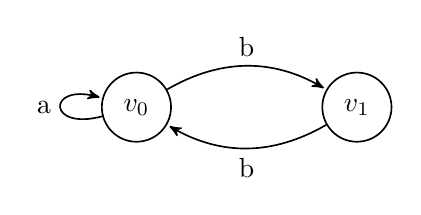
\begin{tikzpicture}[->,>=stealth',shorten >=1pt,auto,node distance=2.8cm, semithick]

    \node[state] (A)                    {$v_0$};
    \node[state]         (B) [right of=A] {$v_1$};
    
    \path (A) edge  [loop left] node {a} (A)
                edge  [bend left] node {b} (B)
            (B) edge  [bend left] node {b} (A);
    \end{tikzpicture}

    \caption{Input graph.}
    \label{fig:input-graph}

\end{figure}

\begin{figure}
    \centering
    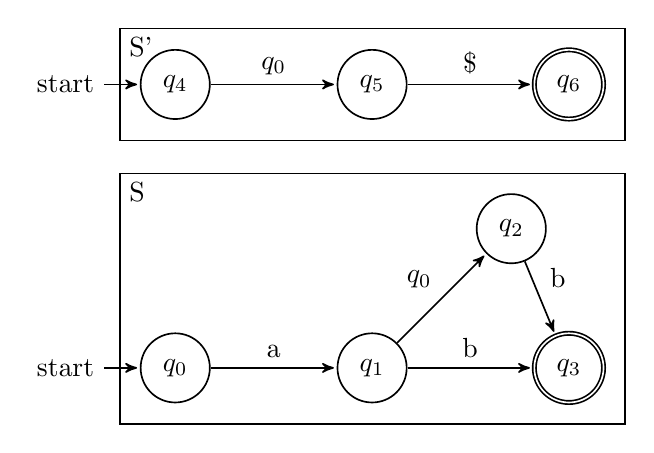
\begin{tikzpicture}[->,>=stealth',shorten >=1pt,auto,node distance=2.5cm, semithick]

    \node[initial,state]   (F)              {$q_4$};
    \node[state]           (G) [right of=F] {$q_5$};
    \node[accepting,state] (H) [right of=G] {$q_6$};
    \node[draw=black, fit= (F) (G) (H), inner sep=0.25cm] (J) {};
    \node[below right] at (J.north west) {S'};

    \path (F) edge              node {$q_0$} (G)
            (G) edge              node {$\$$} (H); 

    \node[initial,state] (A) [below = 2.7cm of F] {$q_0$};
    \node[state]         (B) [right of=A] {$q_1$};
    \node[state]         (D) [above right of=B] {$q_2$};
    \node[accepting,state]         (C) [right of=B] {$q_3$};
    \node [draw=black, fit= (A) (C) (D), inner sep=0.25cm] (E) {};
    \node[below right] at (E.north west) {S};

    \path (A) edge              node {a} (B)
            (B) edge              node {$q_0$} (D)
                edge              node {b} (C)
            (D) edge              node {b} (C);
    \end{tikzpicture}
    
    \caption{Extended RSM for grammar $S \to a \ b \mid a \ S \ b$. We automatically add the rule $S' \to S \ \$ $ to simplify query processing termination condition.}
    \label{fig:example-rsm}
\end{figure}

The resulting SPPF is shown in Fig.~\ref{fig:SPPF}.
Its root is the node $R^{q_4,v_0}_{q_5,v_0}$, which indicates that it represents paths from $v_0$ to $v_0$ that can be recognized by the RSM transitioning from state $q_4$ to $q_5$.
This transition corresponds to recognizing a word derived from the nonterminal $S$.
The node $R^{q_0,v_0}_{q_3,v_0}$ is the entry point for a cycle.
The node $R^{q_0,v_0}_{q_3,v_1}$ has two siblings, indicating two ways to construct the corresponding subpath.
The first corresponds to the shortest possible path: $$v_0 \xrightarrow{a} v_0 \xrightarrow{a} v_0 \xrightarrow{b} v_1 \xrightarrow{b} v_0.$$
The second contains the cycle mentioned above and therefore represents an infinite family of paths formed by repeatedly wrapping the shortest path with additional pairs of $a$s and $b$s.
For example, traversing the cycle once yields the path: $$v_0 \xrightarrow{a} v_0 \xrightarrow{a} v_0 \xrightarrow{a} v_0 \xrightarrow{a} v_0 \xrightarrow{b} v_1 \xrightarrow{b} v_0 \xrightarrow{b} v_1 \xrightarrow{b} v_0.$$

\begin{figure}[htbp] 
    \centering
    \resizebox{1\textwidth}{!}{
    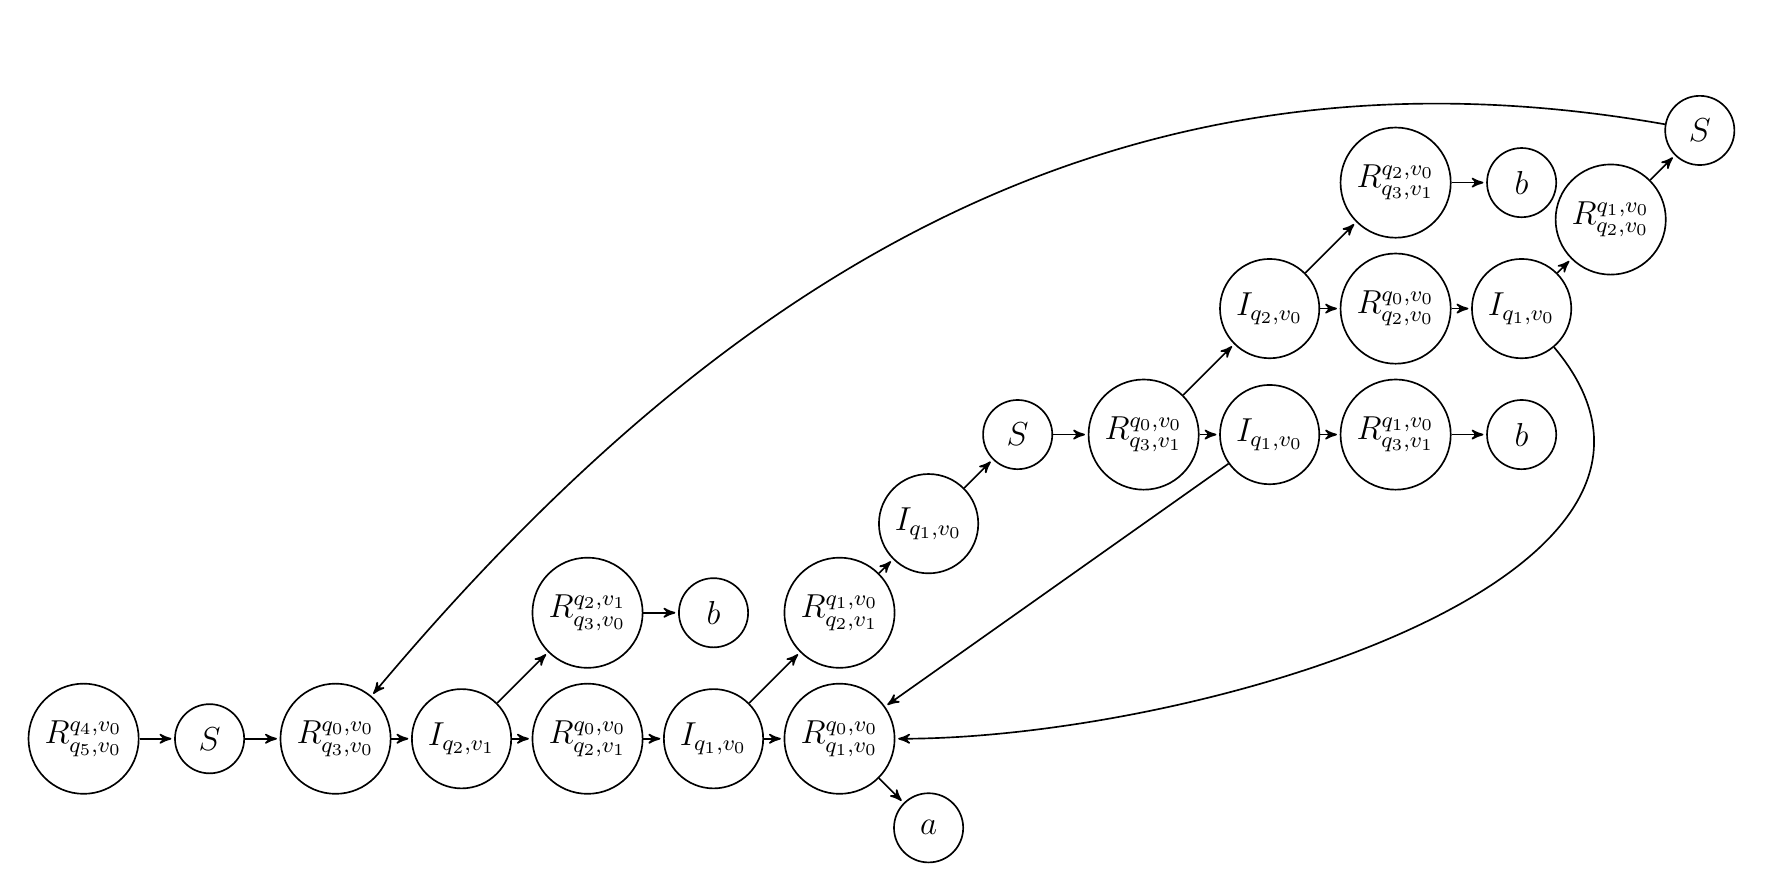
\begin{tikzpicture}[->,>=stealth',shorten >=1pt,auto,node distance=1.6cm, semithick, every node/.style={font=\large}]

    \node[state]         (A)              {$R^{q_4,v_0}_{q_5,v_0}$};
    \node[state]         (B) [right of=A] {$S$};
    \node[state]         (C) [right of=B] {$R^{q_0,v_0}_{q_3,v_0}$};
    \node[state]         (D) [right of=C] {$I_{q_2,v_1}$};
    \node[state]         (E) [right of=D] {$R^{q_0,v_0}_{q_2,v_1}$};
    \node[state]         (F) [above of=E] {$R^{q_2,v_1}_{q_3,v_0}$}; 	
    \node[state]         (G) [right of=E] {$I_{q_1,v_0}$};
    \node[state]         (H) [right of=F] {$b$};
    \node[state]         (J) [right of=G] {$R^{q_0,v_0}_{q_1,v_0}$};
    \node[state]         (I) [above of=J] {$R^{q_1,v_0}_{q_2,v_1}$};
    \node[state]         (K) [below right of=J] {$a$};
    \node[state]         (L) [above right of=I] {$I_{q_1,v_0}$};
    \node[state]         (M) [above right of=L] {$S$};
    \node[state]         (N) [right of=M] {$R^{q_0,v_0}_{q_3,v_1}$};
    \node[state]         (O) [right of=N] {$I_{q_1,v_0}$};
    \node[state]         (P) [above of=O] {$I_{q_2,v_0}$};
    \node[state]         (R) [right of=P] {$R^{q_0,v_0}_{q_2,v_0}$};
    \node[state]         (S) [above of=R] {$R^{q_2,v_0}_{q_3,v_1}$};
    \node[state]         (T) [right of=O] {$R^{q_1,v_0}_{q_3,v_1}$};
    \node[state]         (U) [right of=T] {$b$};
    \node[state]         (V) [right of=S] {$b$};
    \node[state]         (W) [right of=R] {$I_{q_1,v_0}$};
    %\node[state]         (X) [right of=O] {$R^{q_0,v_0}_{q_1,v_0}$};
    \node[state]         (X) [above right of=W] {$R^{q_1,v_0}_{q_2,v_0}$};
    \node[state]         (Y) [above right of=X] {$S$};
    
    \path (A) edge          (B)
            (B) edge   (C)
            (C) edge   (D)
            (D) edge   (E)
            (D) edge   (F)
            (E) edge   (G)
            (F) edge   (H)
            (G) edge   (J)
            (G) edge   (I)
            (J) edge   (K)
            (I) edge   (L)
            (L) edge   (M)
            (M) edge   (N)
            (N) edge   (O)
            (N) edge   (P)
            (O) edge   (J)
            (O) edge   (T)
            (P) edge   (R)
            (R) edge   (W)
            (P) edge   (S)
            (T) edge   (U)
            (S) edge   (V)
            (W) edge[in=0, out=310]   (J)
            (W) edge   (X)
            (X) edge   (Y)
            (Y) edge[in=50, out=170]   (C)
            
            ;
    \end{tikzpicture}
    }
    \caption{The SPPF restored from the path index represented in~\ref{fig:sppf-matrix} for all paths from $v_0$ to $v_0$.}
    \label{fig:SPPF}
\end{figure}



\documentclass[
11pt,%
tightenlines,%
twoside,%
onecolumn,%
nobibnotes,%
nofootinbib,%
superscriptaddress,%
noshowpacs,%
centertags]%
{revtex4-2}
\usepackage{ljm}
\setcaptionwidth{0.93\textwidth}

% --- ГРАФИКА (WINDOWS) ---
\usepackage{epstopdf} % Критично для Windows: конвертирует EPS на лету
\graphicspath{{figures/}} 

% --- СТИЛЬ ЖУРНАЛА ---
\usepackage{ljm} % Файл должен лежать рядом!

% --- МАТЕМАТИКА И ТАБЛИЦЫ ---
\usepackage{mathtools}
\usepackage{colortbl}
\usepackage{algorithm2e}
% \usepackage{multirow}
\usepackage{makecell}  %new line in one table cell

% --- TIKZ (ВНИМАНИЕ: Для журнала в итоге нужны EPS файлы) ---
\usepackage{pgf}
\usepackage{tikz}
\usepackage{nicematrix}
\usetikzlibrary{arrows, automata, fit, calc, positioning}

% --- ДОПОЛНИТЕЛЬНО ---
% \usepackage{soul}
\usepackage[makeroom]{cancel}
\newcommand{\mycomment}[1]{}

\usepackage[caption=false]{subfig}
\usepackage{wrapfig}

\begin{document}
%
\title{GLL-based Context-Free Path Querying for Neo4j}

% --- АВТОРЫ (Формат RevTeX) ---

\author{Vadim Abzalov}
\email[E-mail: ]{vadim.i.abzalov@gmail.com}
\affiliation{Saint Petersburg State University, St. Petersburg, Russia}

\author{Vlada Pogozhelskaya}
\email[E-mail: ]{vvpogozhelskaia@edu.hse.ru}
\affiliation{National Research University Higher School of Economics, St. Petersburg, Russia}

\author{Vladimir Kutuev}
\email[E-mail: ]{v.kutuev@spbu.ru}
\affiliation{Saint Petersburg State University, St. Petersburg, Russia}

\author{Olga Bachishche}
\email[E-mail: ]{bachisheo@gmail.com}
\affiliation{ITMO University, St. Petersburg, Russia}

\author{Semyon Grigorev}
\email[E-mail: ]{s.v.grigoriev@spbu.ru}
\affiliation{Saint Petersburg State University, St. Petersburg, Russia}


% --- АННОТАЦИЯ (Должна быть ДО maketitle) ---
\begin{abstract}
We propose a GLL-based \textit{context-free path querying} algorithm that handles queries in Extended Backus-Naur Form (EBNF) using Recursive State Machines (RSM). Utilization of EBNF allows one to combine traditional regular expressions and mutually recursive patterns in constraints natively. The proposed algorithm solves both the \textit{reachability-only} and the \textit{all-paths} problems for the \textit{all-pairs} and the \textit{multiple sources} cases. The evaluation on real-world graphs demonstrates that the utilization of RSMs increases the performance of query evaluation. Being implemented as a stored procedure for Neo4j, our solution demonstrates better performance than a similar solution for RedisGraph. The performance of our solution on regular path queries is comparable to the performance of the native Neo4j solution, and in some cases, our solution requires significantly less memory.
\end{abstract}

% --- КЛЮЧЕВЫЕ СЛОВА ---
\keywords{Graph database, graph querying, context-free path querying, CFPQ, reachability problem, all-paths problem, generalized LL, GLL}

% --- ГЕНЕРАЦИЯ ЗАГОЛОВКА ---
\maketitle
\renewcommand{\figurename}{Fig.} 
% --- MAIN CONTENT ---
\section{Introduction}

Context-free path querying (CFPQ) allows one to use context-free grammars to specify constraints on paths in edge-labeled graphs. Compared to regular path queries (RPQ), CFPQ is strictly more expressive: for instance, a context-free grammar can be built to find siblings or same-generation categories in a taxonomy~\cite{Azimov:2018:CPQ:3210259.3210264,Kuijpers:2019:ESC:3335783.3335791}. This expressiveness allows CFPQ to be used for graph analysis in such areas as bioinformatics (hierarchy analysis~\cite{zhangCfPgRdf}, similarity queries~\cite{SubgraphQueriesbyContextfreeGrammars}), data provenance analysis~\cite{8731467}, static code analysis~\cite{Zheng,10.1145/373243.360208}. Although a lot of algorithms for CFPQ have been proposed, poor performance on real-world graphs and bad integration with real-world graph databases and graph analysis systems are still problems that hinder the adoption of CFPQ.

The problem with the performance of the CFPQ algorithms in real-world scenarios was pointed out by Jochem Kuijpers~\cite{Kuijpers:2019:ESC:3335783.3335791} as a result of an attempt to extend the Neo4j graph database with CFPQ. Several algorithms, based on such techniques as LR parsing algorithm~\cite{santosBottomUp}, dynamic programming~\cite{hellingsRelational}, LL parsing algorithm~\cite{10.1145/3167132.3167265}, linear algebra~\cite{Azimov:2018:CPQ:3210259.3210264}, were implemented, using Neo4j as a graph storage, and evaluated. None of them were performant enough to be used in real-world applications.   

Since Jochem Kuijpers pointed out the performance problem, it was shown that linear-algebra-based CFPQ algorithms, which operate over the adjacency matrix of the input graph and utilize parallel algorithms for linear algebraic operations, demonstrate good performance~\cite{10.1145/3398682.3399163}. Moreover, the matrix-based CFPQ algorithm is a base for the first full-stack support of CFPQ by extending the RedisGraph graph database~\cite{10.1145/3398682.3399163}.  

However, adjacency matrix is not the only possible format for graph representation, and data format conversion may take a lot of time; thus, it is not applicable in some cases. As a result, the development of the performant CFPQ algorithm for graph representations not based on matrices and its integration with real-world graph databases is still an open problem. Moreover, while the \textit{all pairs context-free constrained reachability} is widely discussed in the community, such practical cases as the \textit{all-paths} queries and the \textit{multiple sources} queries are not studied enough.

Additionally, almost all existing solutions are for \textit{reachability-only} problem. Recently, Jelle Hellings in~\cite{Hellings2020ExplainingPQ} and Rustam Azimov in~\cite{10.1145/3461837.3464513} have proposed algorithms that allow one to extract paths that satisfy the specified context-free constraints. The ability to extract paths of interest is important for some applications where the user wants to know not only the fact that one vertex is reachable from another one, but also to get a detailed explanation of why this vertex is reachable. One of such applications is a program code analysis where the fact is a potential problem in code, and paths can help to analyze and fix this problem. While the utilization of the general-purpose graph databases for code analysis is gaining popularity~\cite{9064792}, CFPQ algorithms that provide a structural representation of paths are not studied enough. 

Generalized LL (GLL) is a parsing algorithm that can handle any context-free grammar, including left-recursive and ambiguous ones. Similar to GLR (e.g. Tomita algorithm), it achieves this by using a graph-structured stack (GSS) to efficiently share and manage the parsing state, allowing it to explore all possible derivations in parallel without an exponential time cost. The output of the parsing is a compact representation of all possible parse trees for the input, known as a \textit{parse forest}. It was shown that the GLL algorithm can be naturally generalized to the CFPQ algorithm~\cite{Grigorev:2017:CPQ:3166094.3166104}. Moreover, this provides a natural solution not only for the \textit{reachability-only} problem but also for the \textit{all-paths} problem. At the same time, there exists a high-performance GLL parsing algorithm~\cite{AfroozenFasterGll} and its implementation in the Iguana project~\cite{iguana-parser}. 

Additionally, pure context-free grammars in Backus-Naur Form (BNF) are too verbose to express complex constraints. However, almost all algorithms require a query to be in such form. At the same time, Extended Backus-Naur Form (EBNF) can be used to specify context-free languages. EBNF allows combining typical regular expressions with mutually recursive rules which are required to specify context-free languages. That makes EBNF more user-friendly. But there are no CFPQ algorithms that utilize EBNF for query specification.

In this paper, we generalize the GLL parsing algorithm to handle queries in EBNF without its transformation. We show that it allows us to increase the performance of the query evaluation. We also integrate our solution with the Neo4j graph database and evaluate it. Thus, we make the following contributions in this paper.
\begin{itemize}
    \item We propose the GLL-based CFPQ algorithm that can handle queries in Extended Backus-Naur Form without transformation. Our solution utilizes Recursive State Machines (RSM)~\cite{10.1145/1075382.1075387} for it. The proposed algorithm can be used to solve both the \textit{reachability-only} and the \textit{all-paths} problems.
    \item We provide an implementation of the proposed CFPQ algorithm. By experimental study on real-world graphs we show that utilization of RSMs allows one to increase performance of the query evaluation. 
    \item We integrate the implemented algorithm with Neo4j by providing a respective stored procedure that can be called from Cypher. Currently, we use Neo4j as a graph storage and do not extend Cypher to express context-free path patterns. Thus, expressive power of our solution is limited: we cannot use the full power of Cypher within our constraints. Implementing a query language extension amounts to a lot of additional effort and is a part of future work.
    \item We evaluate the proposed solution on several real-world graphs. Our evaluation shows that the proposed solution in order of magnitude is faster than a similar linear algebra-based solution for RedisGraph. Moreover, we show that our solution is compatible with native Neo4j solution for RPQs, and in some cases requires significantly less memory. Note that while Cypher's expressively is limited, our solution can handle arbitrary RPQs.
\end{itemize}

The paper has the following structure. In section~\ref{section:preliminaries} we introduce basic notions and definitions from graph theory and formal language theory. Then, in section~\ref{section:RSM} we introduce \textit{recursive state machines} and provide an example of the CFPQ evaluation using na{\"{\i}}ve strategy which may lead to infinite computations. Section~\ref{section:GLL-CFPQ} contains a description of the GLL-based CFPQ evaluation algorithm which uses RSM and solves problems of the na{\"{\i}}ve strategy from the previous section: the algorithm always terminates and can build a finite representation of all paths of interest. Section~\ref{section:dataset} introduces a data set (both graphs and queries) which will be used further for experiments. Further, in section~\ref{section:BFN_or_RSM} we use this data set to compare different versions of the GLL-based CFPQ algorithm. After that, in section~\ref{section:cfpq_for_neo4j} we provide details on the integration of the best version into the Neo4j graph database, and evaluate our solution on the data set introduced before. Related work is discussed in section~\ref{section:related_work}. Final remarks and conclusion are provided in section~\ref{section:conclusion}.
\section{Preliminaries}\label{section:preliminaries}

In this section, we introduce basic definitions and notations for graphs, regular languages, context-free grammars, and finally, we formulate variants of the FLPQ problem.

We use a directed edge-labelled graph as a data model. We denote a graph as $D=\langle V,E,L \rangle$, where $V$ is a finite set of vertices, $E \subseteq V \times L \times V$ is a set of edges, and $L$ is a set of edge labels. A path $\pi$ in a graph $D$ is a sequence of edges: $u  \xrightarrow{l_0} \ldots \xrightarrow{l_m} v$. We denote a path between vertices $u$ and $v$ as $u\pi v$. The function $\omega$ maps a path to a word by concatenating the labels of its edges:
\begin{equation}\label{eqn:omega}
  \omega(\pi) = \omega(u \xrightarrow{l_0} \ldots \xrightarrow{l_m} v) = l_0\ldots l_m .  
\end{equation}

In the context of formal languages, we would like to remind the reader of some fundamental facts about regular expressions and regular languages.

\begin{definition}
    A \textit{regular expression} over the alphabet $\Sigma$ specifies a \textit{regular language} using the following syntax.
    \begin{itemize}
        \item If $t \in \Sigma$, then $t$ is a regular expression.
        \item The concatenation $E_1 \cdot E_2$ of two regular expressions $E_1$ and $E_2$ is a regular expression. Note that in some cases $\cdot$ may be omitted.
        \item The union $E_1 \mid E_2$ of two regular expressions $E_1$ and $E_2$ is a regular expression.
        \item The Kleene star $E^* = \bigcup_{n=0}^{n=\infty} R^n$ of a regular expression $E$ is a regular expression.
    \end{itemize}
\end{definition}

In some cases $E^+$ can be used as syntactic sugar for $E \cdot E^*$. 

Both regular expressions and finite automata specify regular languages and can be converted into each other. Every regular language can be specified using deterministic finite automata without $\varepsilon$-transitions. Note that regular languages form a strong subset of the context-free languages.

\begin{definition}\label{def:bnf}
A \textit{context-free grammar} is a 4-tuple $G=\langle \Sigma, \mathcal{N}, P, S\rangle$, where $\Sigma$ is a finite set of terminals, $\mathcal{N}$ is a finite set of nonterminals, $S \in N$ is the start nonterminal, and $P$ is a set of productions. Each production has the following form: $N_i \to w$, where $N_i \in \mathcal{N}$ is the left-hand side of the production, and $w \in (\Sigma \cup \mathcal{N} )^*$ is the right-hand side of the production.    
\end{definition}
 
 For simplicity, $S \to w_1 \mid w_2$ is used instead of $S \to w_1; S \to w_2$. Some grammar examples are presented in equations~\ref{eqn:g_1},~\ref{eqn:g_2}, and~\ref{eqn:geo}. 

 \begin{definition}
 A \textit{derivation step} (in the grammar $G =\langle \Sigma, \mathcal{N}, P, S\rangle$) is a production application: having a sequence of form $w_1N_0w_2$, where $N_0 \in \mathcal{N}$ and $w_1, w_2 \in (\Sigma \cup \mathcal{N})^*$, and a production $N_0 \to w_3$, one gets a sequence $w_1w_3w_2$, by replacing the left-hand side of the production with its right-hand side.    
 \end{definition}

\begin{definition}
A word $w \in \Sigma^*$ is \textit{derivable} in the grammar $G=\langle \Sigma, \mathcal{N}, P, S\rangle$ if there is a sequence of derivation steps such that the initial sequence is the start nonterminal of the grammar and $w$ is a final sequence: $S \to w_1 \to \ldots \to w$, or $S \to^* w$. 
\end{definition}

\begin{definition}
The \textit{language specified by the context-free grammar} $G=\langle \Sigma, \mathcal{N}, P, S\rangle$ (denoted $\mathcal{L}(G)$) is a set of words derivable from the start nonterminal of the given grammar: $\mathcal{L}(G) = \{ w \mid S \to ^* w \}$.
\end{definition}

\begin{definition}\label{def:ebnf}
    A context-free grammar $G=\langle \Sigma, \mathcal{N}, P, S\rangle$ is in \textit{Extended Backus-Naur Form} (EBNF) if productions have the form $\mathcal{N} \to E$ where $E$ is a regular expression over $\mathcal{N} \cup \Sigma$.
\end{definition}

Grammar in EBNF can be converted to Backus-Naur Form, but such transformation requires introducing new productions and new nonterminals, which leads to a significant increase in the size of the grammar and, subsequently, poor performance of the path querying algorithms.  

We use a generalization of a \textit{parse tree} to represent the result of the query.

\begin{definition}
    \textit{Parse tree} of the sequence $w$ w.r.t. the context-free grammar $G=\langle \Sigma, \mathcal{N}, P, S\rangle$ in EBNF is a rooted, node-labelled, ordered tree with the following properties.
    \begin{itemize}
        \item All leaves are labelled with the elements of $\Sigma \cup \{\varepsilon\}$, where $\varepsilon \notin \Sigma \cup \mathcal{N}$ is a special symbol to denote the empty string. Left-to-right concatenation of leaves forms $w$.
        \item All other nodes are labelled with the elements of $\mathcal{N}$.
        \item The root is labelled with $S$.
        \item Let $w_0$ be an ordered concatenation of child's labels of node labelled with $N_i$. Then $w_0 \in \mathcal{L}(r)$, where $N_i \to r \in P$.  
    \end{itemize}
\end{definition}

A set of problems for the graph $D$ and the language $\mathcal{L}$ can be formulated: 
\begin{align}
R &= \{(u,v) \mid \text{exists a path } u\pi v \text{ in } D, \omega(\pi) \in \mathcal{L}  \} \label{eqn:all_pairs_reachability}
\\
Q &= \{\pi \mid \text{exists a path } u\pi v \text{ in } D, \omega(\pi) \in \mathcal{L}  \} \label{eqn:all_pairs_all_paths}
\\
R(I) &= \{(u,v) \mid \text{exists a path } u\pi v \text{ in } D, u \in I, \omega(\pi) \in \mathcal{L}  \} \label{eqn:multiple_source_reachability}
\\
Q(I) &= \{\pi \mid \text{exists a path } u\pi v \text{ in } D, u \in I, \omega(\pi) \in \mathcal{L}  \} \label{eqn:multiple_source_all_paths}
\end{align}

Here~\ref{eqn:all_pairs_reachability} is the \textit{all-pairs reachability problem}, and~\ref{eqn:all_pairs_all_paths} is the \textit{all-pairs all-paths problem}. The additional parameter $I$ denotes the set of start vertices in~\ref{eqn:multiple_source_reachability} and~\ref{eqn:multiple_source_all_paths}. Thus~\ref{eqn:multiple_source_reachability} and~\ref{eqn:multiple_source_all_paths} --- are the \textit{multiple source reachability} and the \textit{multiple source all-paths} problems, respectively. Note that for the \textit{all-paths} problems, the result $Q$ can be an infinite set. Typically, the algorithms for these problems build a finite structure which contains all paths of interest, not the explicit set of the paths. As far as the intersection of a regular and a context-free language is context-free~\cite{MR0151376}, the mentioned finite representation of the result for the reachability problem is a representation of the context-free language.

This work is focused on a context-free language, but the partial case --- regular languages --- is also discussed. This corresponds to two specific cases of the formal language path querying (FLPQ): \textit{Context-Free Path Querying} (CFPQ) and \textit{Regular Path Querying} (RPQ).  
\section{RSM-based CFPQ algorithm}\label{section:RSM}

In this section, we provide background on Recursive State Machines (RSMs) and describe informally how they can specify context-free constraints for path querying in graphs. 
We also describe the main idea behind adopting GLL for an RSM-based CFPQ algorithm.

A \textit{recursive state machine} (RSM)~\cite{10.1145/1075382.1075387} provides a representation of context-free languages in a way resembling finite automata.
It allows us to use a graph-based specification of context-free languages and unify the processing of regular and context-free languages. 
Moreover, RSMs naturally encode grammars in Extended Backus-Naur Form (EBNF), which is often more compact and user-friendly than BNF.

In our work, we modify the GLL-based CFPQ algorithm to handle RSMs instead of grammars in BNF as a query specification.
This modification improves performance and enables native handling of both context-free and regular languages.
A detailed description of the algorithm, including formal definitions of descriptors, GSS, and correctness proofs, is beyond the scope of this paper and can be found in the extended version~\cite{abzalov2023gllbasedcontextfreepathquerying}.

Our solution is based on the generalized LL parsing algorithm~\cite{SCOTT2010177} which was shown to generalize well to graph processing~\cite{Grigorev:2017:CPQ:3166094.3166104}.
To support RSMs as a query specification, we introduce \emph{matched ranges}: each range is defined by two graph vertices (e.g., $u$ and $v$) and two RSM states (e.g., $p$ and $q$).
A matched range of the form $(p,u),(q,v)$ indicates that there exists at least one path from $u$ to $v$ such that its labels form a word accepted by RSM when starting in state $p$ and ending in state $q$.

As a result of parsing, GLL can construct a \textit{Shared Packed Parse Forest} (SPPF)~\cite{SCOTT20131828}, a special data structure which represents all possible derivations of the input in the compressed form.
A Shared Packed Parse Forest (SPPF) was proposed by Jan Rekers in~\cite{rekers1992parser} to represent parse forest without duplication of subtrees. Later, other versions of SPPF were introduced in different generalized parsing algorithms.
For example, GLL can provide the result in the form of \textit{binary subtree sets}~\cite{SCOTT201963}.
As shown in~\cite{Grigorev:2017:CPQ:3166094.3166104}, the SPPF can finitely represent the result of an all-paths query, enabling the recovery of any concrete path.
We employ SPPF with the following types of nodes. 

\begin{itemize}
    \item A \textit{Terminal node} to represent a matched edge label.
    \item A \textit{Nonterminal node} to represent the root of the subtree that corresponds to paths that can be derived from the respective nonterminal.  
    \item An \textit{Intermediate node} which corresponds to the intermediate point used to connect two matched ranges. It has exactly two children (both range nodes) and is denoted $I_{q,v}$, indicating that ranges are joined at point $(q,v)$.
    \item A \textit{Range node} corresponds to a matched range $(p,u),(q,v)$ and is denoted $R^{p,u}_{q,v}$. It encodes all possible derivations of that range and can have arbitrarily many children of any type except range. Range nodes are reusable within the SPPF.
    \item An \textit{Epsilon node} to represent the empty subtree in the case when nonterminal produces the empty string. 
\end{itemize}

\subsection{Example}\label{section:example_of_rsm}

We give a brief example.
Consider the graph as shown in Fig.~\ref{fig:input-graph} and we seek all paths from $v_0$ to $v_0$ that satisfy the constraint specified by the RSM in Fig.~\ref{fig:example-rsm}.
The RSM describes paths of the form $a^n b^n$, where $n > 0$.
Note that there are infinitely many such paths. 
Therefore, the resulting SPPF contain cycles.

\begin{figure}
    \centering
    
    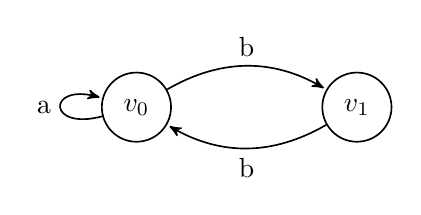
\begin{tikzpicture}[->,>=stealth',shorten >=1pt,auto,node distance=2.8cm, semithick]

    \node[state] (A)                    {$v_0$};
    \node[state]         (B) [right of=A] {$v_1$};
    
    \path (A) edge  [loop left] node {a} (A)
                edge  [bend left] node {b} (B)
            (B) edge  [bend left] node {b} (A);
    \end{tikzpicture}

    \caption{Input graph.}
    \label{fig:input-graph}

\end{figure}

\begin{figure}
    \centering
    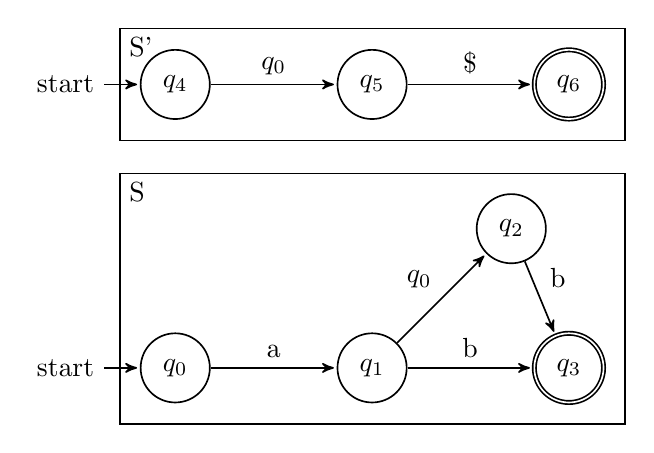
\begin{tikzpicture}[->,>=stealth',shorten >=1pt,auto,node distance=2.5cm, semithick]

    \node[initial,state]   (F)              {$q_4$};
    \node[state]           (G) [right of=F] {$q_5$};
    \node[accepting,state] (H) [right of=G] {$q_6$};
    \node[draw=black, fit= (F) (G) (H), inner sep=0.25cm] (J) {};
    \node[below right] at (J.north west) {S'};

    \path (F) edge              node {$q_0$} (G)
            (G) edge              node {$\$$} (H); 

    \node[initial,state] (A) [below = 2.7cm of F] {$q_0$};
    \node[state]         (B) [right of=A] {$q_1$};
    \node[state]         (D) [above right of=B] {$q_2$};
    \node[accepting,state]         (C) [right of=B] {$q_3$};
    \node [draw=black, fit= (A) (C) (D), inner sep=0.25cm] (E) {};
    \node[below right] at (E.north west) {S};

    \path (A) edge              node {a} (B)
            (B) edge              node {$q_0$} (D)
                edge              node {b} (C)
            (D) edge              node {b} (C);
    \end{tikzpicture}
    
    \caption{Extended RSM for grammar $S \to a \ b \mid a \ S \ b$. We automatically add the rule $S' \to S \ \$ $ to simplify query processing termination condition.}
    \label{fig:example-rsm}
\end{figure}

The resulting SPPF is shown in Fig.~\ref{fig:SPPF}.
Its root is the node $R^{q_4,v_0}_{q_5,v_0}$, which indicates that it represents paths from $v_0$ to $v_0$ that can be recognized by the RSM transitioning from state $q_4$ to $q_5$.
This transition corresponds to recognizing a word derived from the nonterminal $S$.
The node $R^{q_0,v_0}_{q_3,v_0}$ is the entry point for a cycle.
The node $R^{q_0,v_0}_{q_3,v_1}$ has two siblings, indicating two ways to construct the corresponding subpath.
The first corresponds to the shortest possible path: $$v_0 \xrightarrow{a} v_0 \xrightarrow{a} v_0 \xrightarrow{b} v_1 \xrightarrow{b} v_0.$$
The second contains the cycle mentioned above and therefore represents an infinite family of paths formed by repeatedly wrapping the shortest path with additional pairs of $a$s and $b$s.
For example, traversing the cycle once yields the path: $$v_0 \xrightarrow{a} v_0 \xrightarrow{a} v_0 \xrightarrow{a} v_0 \xrightarrow{a} v_0 \xrightarrow{b} v_1 \xrightarrow{b} v_0 \xrightarrow{b} v_1 \xrightarrow{b} v_0.$$

\begin{figure}[htbp] 
    \centering
    \resizebox{1\textwidth}{!}{
    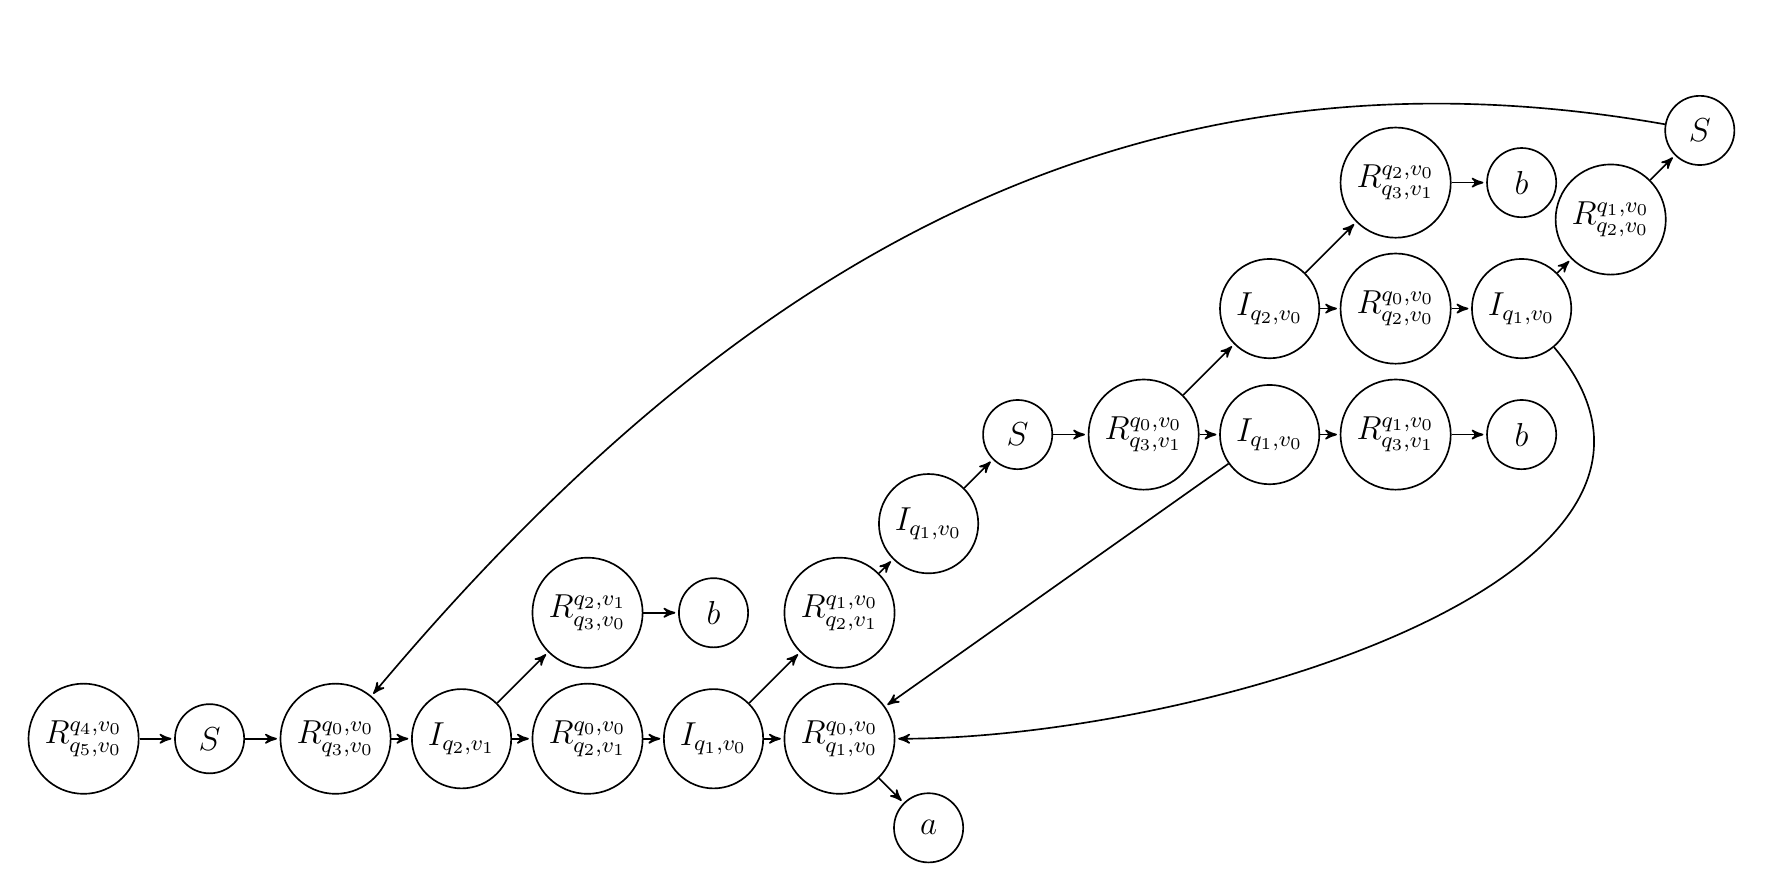
\begin{tikzpicture}[->,>=stealth',shorten >=1pt,auto,node distance=1.6cm, semithick, every node/.style={font=\large}]

    \node[state]         (A)              {$R^{q_4,v_0}_{q_5,v_0}$};
    \node[state]         (B) [right of=A] {$S$};
    \node[state]         (C) [right of=B] {$R^{q_0,v_0}_{q_3,v_0}$};
    \node[state]         (D) [right of=C] {$I_{q_2,v_1}$};
    \node[state]         (E) [right of=D] {$R^{q_0,v_0}_{q_2,v_1}$};
    \node[state]         (F) [above of=E] {$R^{q_2,v_1}_{q_3,v_0}$}; 	
    \node[state]         (G) [right of=E] {$I_{q_1,v_0}$};
    \node[state]         (H) [right of=F] {$b$};
    \node[state]         (J) [right of=G] {$R^{q_0,v_0}_{q_1,v_0}$};
    \node[state]         (I) [above of=J] {$R^{q_1,v_0}_{q_2,v_1}$};
    \node[state]         (K) [below right of=J] {$a$};
    \node[state]         (L) [above right of=I] {$I_{q_1,v_0}$};
    \node[state]         (M) [above right of=L] {$S$};
    \node[state]         (N) [right of=M] {$R^{q_0,v_0}_{q_3,v_1}$};
    \node[state]         (O) [right of=N] {$I_{q_1,v_0}$};
    \node[state]         (P) [above of=O] {$I_{q_2,v_0}$};
    \node[state]         (R) [right of=P] {$R^{q_0,v_0}_{q_2,v_0}$};
    \node[state]         (S) [above of=R] {$R^{q_2,v_0}_{q_3,v_1}$};
    \node[state]         (T) [right of=O] {$R^{q_1,v_0}_{q_3,v_1}$};
    \node[state]         (U) [right of=T] {$b$};
    \node[state]         (V) [right of=S] {$b$};
    \node[state]         (W) [right of=R] {$I_{q_1,v_0}$};
    %\node[state]         (X) [right of=O] {$R^{q_0,v_0}_{q_1,v_0}$};
    \node[state]         (X) [above right of=W] {$R^{q_1,v_0}_{q_2,v_0}$};
    \node[state]         (Y) [above right of=X] {$S$};
    
    \path (A) edge          (B)
            (B) edge   (C)
            (C) edge   (D)
            (D) edge   (E)
            (D) edge   (F)
            (E) edge   (G)
            (F) edge   (H)
            (G) edge   (J)
            (G) edge   (I)
            (J) edge   (K)
            (I) edge   (L)
            (L) edge   (M)
            (M) edge   (N)
            (N) edge   (O)
            (N) edge   (P)
            (O) edge   (J)
            (O) edge   (T)
            (P) edge   (R)
            (R) edge   (W)
            (P) edge   (S)
            (T) edge   (U)
            (S) edge   (V)
            (W) edge[in=0, out=310]   (J)
            (W) edge   (X)
            (X) edge   (Y)
            (Y) edge[in=50, out=170]   (C)
            
            ;
    \end{tikzpicture}
    }
    \caption{The SPPF restored from the path index represented in~\ref{fig:sppf-matrix} for all paths from $v_0$ to $v_0$.}
    \label{fig:SPPF}
\end{figure}



\documentclass[
11pt,%
tightenlines,%
twoside,%
onecolumn,%
nobibnotes,%
nofootinbib,%
superscriptaddress,%
noshowpacs,%
centertags]%
{revtex4-2}
\usepackage{ljm}
\setcaptionwidth{0.93\textwidth}

% --- ГРАФИКА (WINDOWS) ---
\usepackage{epstopdf} % Критично для Windows: конвертирует EPS на лету
\graphicspath{{figures/}} 

% --- СТИЛЬ ЖУРНАЛА ---
\usepackage{ljm} % Файл должен лежать рядом!

% --- МАТЕМАТИКА И ТАБЛИЦЫ ---
\usepackage{mathtools}
\usepackage{colortbl}
\usepackage{algorithm2e}
% \usepackage{multirow}
\usepackage{makecell}  %new line in one table cell

% --- TIKZ (ВНИМАНИЕ: Для журнала в итоге нужны EPS файлы) ---
\usepackage{pgf}
\usepackage{tikz}
\usepackage{nicematrix}
\usetikzlibrary{arrows, automata, fit, calc, positioning}

% --- ДОПОЛНИТЕЛЬНО ---
% \usepackage{soul}
\usepackage[makeroom]{cancel}
\newcommand{\mycomment}[1]{}

\usepackage[caption=false]{subfig}
\usepackage{wrapfig}

\begin{document}
%
\title{GLL-based Context-Free Path Querying for Neo4j}

% --- АВТОРЫ (Формат RevTeX) ---

\author{Vadim Abzalov}
\email[E-mail: ]{vadim.i.abzalov@gmail.com}
\affiliation{Saint Petersburg State University, St. Petersburg, Russia}

\author{Vlada Pogozhelskaya}
\email[E-mail: ]{vvpogozhelskaia@edu.hse.ru}
\affiliation{National Research University Higher School of Economics, St. Petersburg, Russia}

\author{Vladimir Kutuev}
\email[E-mail: ]{v.kutuev@spbu.ru}
\affiliation{Saint Petersburg State University, St. Petersburg, Russia}

\author{Olga Bachishche}
\email[E-mail: ]{bachisheo@gmail.com}
\affiliation{ITMO University, St. Petersburg, Russia}

\author{Semyon Grigorev}
\email[E-mail: ]{s.v.grigoriev@spbu.ru}
\affiliation{Saint Petersburg State University, St. Petersburg, Russia}


% --- АННОТАЦИЯ (Должна быть ДО maketitle) ---
\begin{abstract}
We propose a GLL-based \textit{context-free path querying} algorithm that handles queries in Extended Backus-Naur Form (EBNF) using Recursive State Machines (RSM). Utilization of EBNF allows one to combine traditional regular expressions and mutually recursive patterns in constraints natively. The proposed algorithm solves both the \textit{reachability-only} and the \textit{all-paths} problems for the \textit{all-pairs} and the \textit{multiple sources} cases. The evaluation on real-world graphs demonstrates that the utilization of RSMs increases the performance of query evaluation. Being implemented as a stored procedure for Neo4j, our solution demonstrates better performance than a similar solution for RedisGraph. The performance of our solution on regular path queries is comparable to the performance of the native Neo4j solution, and in some cases, our solution requires significantly less memory.
\end{abstract}

% --- КЛЮЧЕВЫЕ СЛОВА ---
\keywords{Graph database, graph querying, context-free path querying, CFPQ, reachability problem, all-paths problem, generalized LL, GLL}

% --- ГЕНЕРАЦИЯ ЗАГОЛОВКА ---
\maketitle
\renewcommand{\figurename}{Fig.} 
% --- MAIN CONTENT ---
\section{Introduction}

Context-free path querying (CFPQ) allows one to use context-free grammars to specify constraints on paths in edge-labeled graphs. Compared to regular path queries (RPQ), CFPQ is strictly more expressive: for instance, a context-free grammar can be built to find siblings or same-generation categories in a taxonomy~\cite{Azimov:2018:CPQ:3210259.3210264,Kuijpers:2019:ESC:3335783.3335791}. This expressiveness allows CFPQ to be used for graph analysis in such areas as bioinformatics (hierarchy analysis~\cite{zhangCfPgRdf}, similarity queries~\cite{SubgraphQueriesbyContextfreeGrammars}), data provenance analysis~\cite{8731467}, static code analysis~\cite{Zheng,10.1145/373243.360208}. Although a lot of algorithms for CFPQ have been proposed, poor performance on real-world graphs and bad integration with real-world graph databases and graph analysis systems are still problems that hinder the adoption of CFPQ.

The problem with the performance of the CFPQ algorithms in real-world scenarios was pointed out by Jochem Kuijpers~\cite{Kuijpers:2019:ESC:3335783.3335791} as a result of an attempt to extend the Neo4j graph database with CFPQ. Several algorithms, based on such techniques as LR parsing algorithm~\cite{santosBottomUp}, dynamic programming~\cite{hellingsRelational}, LL parsing algorithm~\cite{10.1145/3167132.3167265}, linear algebra~\cite{Azimov:2018:CPQ:3210259.3210264}, were implemented, using Neo4j as a graph storage, and evaluated. None of them were performant enough to be used in real-world applications.   

Since Jochem Kuijpers pointed out the performance problem, it was shown that linear-algebra-based CFPQ algorithms, which operate over the adjacency matrix of the input graph and utilize parallel algorithms for linear algebraic operations, demonstrate good performance~\cite{10.1145/3398682.3399163}. Moreover, the matrix-based CFPQ algorithm is a base for the first full-stack support of CFPQ by extending the RedisGraph graph database~\cite{10.1145/3398682.3399163}.  

However, adjacency matrix is not the only possible format for graph representation, and data format conversion may take a lot of time; thus, it is not applicable in some cases. As a result, the development of the performant CFPQ algorithm for graph representations not based on matrices and its integration with real-world graph databases is still an open problem. Moreover, while the \textit{all pairs context-free constrained reachability} is widely discussed in the community, such practical cases as the \textit{all-paths} queries and the \textit{multiple sources} queries are not studied enough.

Additionally, almost all existing solutions are for \textit{reachability-only} problem. Recently, Jelle Hellings in~\cite{Hellings2020ExplainingPQ} and Rustam Azimov in~\cite{10.1145/3461837.3464513} have proposed algorithms that allow one to extract paths that satisfy the specified context-free constraints. The ability to extract paths of interest is important for some applications where the user wants to know not only the fact that one vertex is reachable from another one, but also to get a detailed explanation of why this vertex is reachable. One of such applications is a program code analysis where the fact is a potential problem in code, and paths can help to analyze and fix this problem. While the utilization of the general-purpose graph databases for code analysis is gaining popularity~\cite{9064792}, CFPQ algorithms that provide a structural representation of paths are not studied enough. 

Generalized LL (GLL) is a parsing algorithm that can handle any context-free grammar, including left-recursive and ambiguous ones. Similar to GLR (e.g. Tomita algorithm), it achieves this by using a graph-structured stack (GSS) to efficiently share and manage the parsing state, allowing it to explore all possible derivations in parallel without an exponential time cost. The output of the parsing is a compact representation of all possible parse trees for the input, known as a \textit{parse forest}. It was shown that the GLL algorithm can be naturally generalized to the CFPQ algorithm~\cite{Grigorev:2017:CPQ:3166094.3166104}. Moreover, this provides a natural solution not only for the \textit{reachability-only} problem but also for the \textit{all-paths} problem. At the same time, there exists a high-performance GLL parsing algorithm~\cite{AfroozenFasterGll} and its implementation in the Iguana project~\cite{iguana-parser}. 

Additionally, pure context-free grammars in Backus-Naur Form (BNF) are too verbose to express complex constraints. However, almost all algorithms require a query to be in such form. At the same time, Extended Backus-Naur Form (EBNF) can be used to specify context-free languages. EBNF allows combining typical regular expressions with mutually recursive rules which are required to specify context-free languages. That makes EBNF more user-friendly. But there are no CFPQ algorithms that utilize EBNF for query specification.

In this paper, we generalize the GLL parsing algorithm to handle queries in EBNF without its transformation. We show that it allows us to increase the performance of the query evaluation. We also integrate our solution with the Neo4j graph database and evaluate it. Thus, we make the following contributions in this paper.
\begin{itemize}
    \item We propose the GLL-based CFPQ algorithm that can handle queries in Extended Backus-Naur Form without transformation. Our solution utilizes Recursive State Machines (RSM)~\cite{10.1145/1075382.1075387} for it. The proposed algorithm can be used to solve both the \textit{reachability-only} and the \textit{all-paths} problems.
    \item We provide an implementation of the proposed CFPQ algorithm. By experimental study on real-world graphs we show that utilization of RSMs allows one to increase performance of the query evaluation. 
    \item We integrate the implemented algorithm with Neo4j by providing a respective stored procedure that can be called from Cypher. Currently, we use Neo4j as a graph storage and do not extend Cypher to express context-free path patterns. Thus, expressive power of our solution is limited: we cannot use the full power of Cypher within our constraints. Implementing a query language extension amounts to a lot of additional effort and is a part of future work.
    \item We evaluate the proposed solution on several real-world graphs. Our evaluation shows that the proposed solution in order of magnitude is faster than a similar linear algebra-based solution for RedisGraph. Moreover, we show that our solution is compatible with native Neo4j solution for RPQs, and in some cases requires significantly less memory. Note that while Cypher's expressively is limited, our solution can handle arbitrary RPQs.
\end{itemize}

The paper has the following structure. In section~\ref{section:preliminaries} we introduce basic notions and definitions from graph theory and formal language theory. Then, in section~\ref{section:RSM} we introduce \textit{recursive state machines} and provide an example of the CFPQ evaluation using na{\"{\i}}ve strategy which may lead to infinite computations. Section~\ref{section:GLL-CFPQ} contains a description of the GLL-based CFPQ evaluation algorithm which uses RSM and solves problems of the na{\"{\i}}ve strategy from the previous section: the algorithm always terminates and can build a finite representation of all paths of interest. Section~\ref{section:dataset} introduces a data set (both graphs and queries) which will be used further for experiments. Further, in section~\ref{section:BFN_or_RSM} we use this data set to compare different versions of the GLL-based CFPQ algorithm. After that, in section~\ref{section:cfpq_for_neo4j} we provide details on the integration of the best version into the Neo4j graph database, and evaluate our solution on the data set introduced before. Related work is discussed in section~\ref{section:related_work}. Final remarks and conclusion are provided in section~\ref{section:conclusion}.
\section{Preliminaries}\label{section:preliminaries}

In this section, we introduce basic definitions and notations for graphs, regular languages, context-free grammars, and finally, we formulate variants of the FLPQ problem.

We use a directed edge-labelled graph as a data model. We denote a graph as $D=\langle V,E,L \rangle$, where $V$ is a finite set of vertices, $E \subseteq V \times L \times V$ is a set of edges, and $L$ is a set of edge labels. A path $\pi$ in a graph $D$ is a sequence of edges: $u  \xrightarrow{l_0} \ldots \xrightarrow{l_m} v$. We denote a path between vertices $u$ and $v$ as $u\pi v$. The function $\omega$ maps a path to a word by concatenating the labels of its edges:
\begin{equation}\label{eqn:omega}
  \omega(\pi) = \omega(u \xrightarrow{l_0} \ldots \xrightarrow{l_m} v) = l_0\ldots l_m .  
\end{equation}

In the context of formal languages, we would like to remind the reader of some fundamental facts about regular expressions and regular languages.

\begin{definition}
    A \textit{regular expression} over the alphabet $\Sigma$ specifies a \textit{regular language} using the following syntax.
    \begin{itemize}
        \item If $t \in \Sigma$, then $t$ is a regular expression.
        \item The concatenation $E_1 \cdot E_2$ of two regular expressions $E_1$ and $E_2$ is a regular expression. Note that in some cases $\cdot$ may be omitted.
        \item The union $E_1 \mid E_2$ of two regular expressions $E_1$ and $E_2$ is a regular expression.
        \item The Kleene star $E^* = \bigcup_{n=0}^{n=\infty} R^n$ of a regular expression $E$ is a regular expression.
    \end{itemize}
\end{definition}

In some cases $E^+$ can be used as syntactic sugar for $E \cdot E^*$. 

Both regular expressions and finite automata specify regular languages and can be converted into each other. Every regular language can be specified using deterministic finite automata without $\varepsilon$-transitions. Note that regular languages form a strong subset of the context-free languages.

\begin{definition}\label{def:bnf}
A \textit{context-free grammar} is a 4-tuple $G=\langle \Sigma, \mathcal{N}, P, S\rangle$, where $\Sigma$ is a finite set of terminals, $\mathcal{N}$ is a finite set of nonterminals, $S \in N$ is the start nonterminal, and $P$ is a set of productions. Each production has the following form: $N_i \to w$, where $N_i \in \mathcal{N}$ is the left-hand side of the production, and $w \in (\Sigma \cup \mathcal{N} )^*$ is the right-hand side of the production.    
\end{definition}
 
 For simplicity, $S \to w_1 \mid w_2$ is used instead of $S \to w_1; S \to w_2$. Some grammar examples are presented in equations~\ref{eqn:g_1},~\ref{eqn:g_2}, and~\ref{eqn:geo}. 

 \begin{definition}
 A \textit{derivation step} (in the grammar $G =\langle \Sigma, \mathcal{N}, P, S\rangle$) is a production application: having a sequence of form $w_1N_0w_2$, where $N_0 \in \mathcal{N}$ and $w_1, w_2 \in (\Sigma \cup \mathcal{N})^*$, and a production $N_0 \to w_3$, one gets a sequence $w_1w_3w_2$, by replacing the left-hand side of the production with its right-hand side.    
 \end{definition}

\begin{definition}
A word $w \in \Sigma^*$ is \textit{derivable} in the grammar $G=\langle \Sigma, \mathcal{N}, P, S\rangle$ if there is a sequence of derivation steps such that the initial sequence is the start nonterminal of the grammar and $w$ is a final sequence: $S \to w_1 \to \ldots \to w$, or $S \to^* w$. 
\end{definition}

\begin{definition}
The \textit{language specified by the context-free grammar} $G=\langle \Sigma, \mathcal{N}, P, S\rangle$ (denoted $\mathcal{L}(G)$) is a set of words derivable from the start nonterminal of the given grammar: $\mathcal{L}(G) = \{ w \mid S \to ^* w \}$.
\end{definition}

\begin{definition}\label{def:ebnf}
    A context-free grammar $G=\langle \Sigma, \mathcal{N}, P, S\rangle$ is in \textit{Extended Backus-Naur Form} (EBNF) if productions have the form $\mathcal{N} \to E$ where $E$ is a regular expression over $\mathcal{N} \cup \Sigma$.
\end{definition}

Grammar in EBNF can be converted to Backus-Naur Form, but such transformation requires introducing new productions and new nonterminals, which leads to a significant increase in the size of the grammar and, subsequently, poor performance of the path querying algorithms.  

We use a generalization of a \textit{parse tree} to represent the result of the query.

\begin{definition}
    \textit{Parse tree} of the sequence $w$ w.r.t. the context-free grammar $G=\langle \Sigma, \mathcal{N}, P, S\rangle$ in EBNF is a rooted, node-labelled, ordered tree with the following properties.
    \begin{itemize}
        \item All leaves are labelled with the elements of $\Sigma \cup \{\varepsilon\}$, where $\varepsilon \notin \Sigma \cup \mathcal{N}$ is a special symbol to denote the empty string. Left-to-right concatenation of leaves forms $w$.
        \item All other nodes are labelled with the elements of $\mathcal{N}$.
        \item The root is labelled with $S$.
        \item Let $w_0$ be an ordered concatenation of child's labels of node labelled with $N_i$. Then $w_0 \in \mathcal{L}(r)$, where $N_i \to r \in P$.  
    \end{itemize}
\end{definition}

A set of problems for the graph $D$ and the language $\mathcal{L}$ can be formulated: 
\begin{align}
R &= \{(u,v) \mid \text{exists a path } u\pi v \text{ in } D, \omega(\pi) \in \mathcal{L}  \} \label{eqn:all_pairs_reachability}
\\
Q &= \{\pi \mid \text{exists a path } u\pi v \text{ in } D, \omega(\pi) \in \mathcal{L}  \} \label{eqn:all_pairs_all_paths}
\\
R(I) &= \{(u,v) \mid \text{exists a path } u\pi v \text{ in } D, u \in I, \omega(\pi) \in \mathcal{L}  \} \label{eqn:multiple_source_reachability}
\\
Q(I) &= \{\pi \mid \text{exists a path } u\pi v \text{ in } D, u \in I, \omega(\pi) \in \mathcal{L}  \} \label{eqn:multiple_source_all_paths}
\end{align}

Here~\ref{eqn:all_pairs_reachability} is the \textit{all-pairs reachability problem}, and~\ref{eqn:all_pairs_all_paths} is the \textit{all-pairs all-paths problem}. The additional parameter $I$ denotes the set of start vertices in~\ref{eqn:multiple_source_reachability} and~\ref{eqn:multiple_source_all_paths}. Thus~\ref{eqn:multiple_source_reachability} and~\ref{eqn:multiple_source_all_paths} --- are the \textit{multiple source reachability} and the \textit{multiple source all-paths} problems, respectively. Note that for the \textit{all-paths} problems, the result $Q$ can be an infinite set. Typically, the algorithms for these problems build a finite structure which contains all paths of interest, not the explicit set of the paths. As far as the intersection of a regular and a context-free language is context-free~\cite{MR0151376}, the mentioned finite representation of the result for the reachability problem is a representation of the context-free language.

This work is focused on a context-free language, but the partial case --- regular languages --- is also discussed. This corresponds to two specific cases of the formal language path querying (FLPQ): \textit{Context-Free Path Querying} (CFPQ) and \textit{Regular Path Querying} (RPQ).  
\section{RSM-based CFPQ algorithm}\label{section:RSM}

In this section, we provide background on Recursive State Machines (RSMs) and describe informally how they can specify context-free constraints for path querying in graphs. 
We also describe the main idea behind adopting GLL for an RSM-based CFPQ algorithm.

A \textit{recursive state machine} (RSM)~\cite{10.1145/1075382.1075387} provides a representation of context-free languages in a way resembling finite automata.
It allows us to use a graph-based specification of context-free languages and unify the processing of regular and context-free languages. 
Moreover, RSMs naturally encode grammars in Extended Backus-Naur Form (EBNF), which is often more compact and user-friendly than BNF.

In our work, we modify the GLL-based CFPQ algorithm to handle RSMs instead of grammars in BNF as a query specification.
This modification improves performance and enables native handling of both context-free and regular languages.
A detailed description of the algorithm, including formal definitions of descriptors, GSS, and correctness proofs, is beyond the scope of this paper and can be found in the extended version~\cite{abzalov2023gllbasedcontextfreepathquerying}.

Our solution is based on the generalized LL parsing algorithm~\cite{SCOTT2010177} which was shown to generalize well to graph processing~\cite{Grigorev:2017:CPQ:3166094.3166104}.
To support RSMs as a query specification, we introduce \emph{matched ranges}: each range is defined by two graph vertices (e.g., $u$ and $v$) and two RSM states (e.g., $p$ and $q$).
A matched range of the form $(p,u),(q,v)$ indicates that there exists at least one path from $u$ to $v$ such that its labels form a word accepted by RSM when starting in state $p$ and ending in state $q$.

As a result of parsing, GLL can construct a \textit{Shared Packed Parse Forest} (SPPF)~\cite{SCOTT20131828}, a special data structure which represents all possible derivations of the input in the compressed form.
A Shared Packed Parse Forest (SPPF) was proposed by Jan Rekers in~\cite{rekers1992parser} to represent parse forest without duplication of subtrees. Later, other versions of SPPF were introduced in different generalized parsing algorithms.
For example, GLL can provide the result in the form of \textit{binary subtree sets}~\cite{SCOTT201963}.
As shown in~\cite{Grigorev:2017:CPQ:3166094.3166104}, the SPPF can finitely represent the result of an all-paths query, enabling the recovery of any concrete path.
We employ SPPF with the following types of nodes. 

\begin{itemize}
    \item A \textit{Terminal node} to represent a matched edge label.
    \item A \textit{Nonterminal node} to represent the root of the subtree that corresponds to paths that can be derived from the respective nonterminal.  
    \item An \textit{Intermediate node} which corresponds to the intermediate point used to connect two matched ranges. It has exactly two children (both range nodes) and is denoted $I_{q,v}$, indicating that ranges are joined at point $(q,v)$.
    \item A \textit{Range node} corresponds to a matched range $(p,u),(q,v)$ and is denoted $R^{p,u}_{q,v}$. It encodes all possible derivations of that range and can have arbitrarily many children of any type except range. Range nodes are reusable within the SPPF.
    \item An \textit{Epsilon node} to represent the empty subtree in the case when nonterminal produces the empty string. 
\end{itemize}

\subsection{Example}\label{section:example_of_rsm}

We give a brief example.
Consider the graph as shown in Fig.~\ref{fig:input-graph} and we seek all paths from $v_0$ to $v_0$ that satisfy the constraint specified by the RSM in Fig.~\ref{fig:example-rsm}.
The RSM describes paths of the form $a^n b^n$, where $n > 0$.
Note that there are infinitely many such paths. 
Therefore, the resulting SPPF contain cycles.

\begin{figure}
    \centering
    
    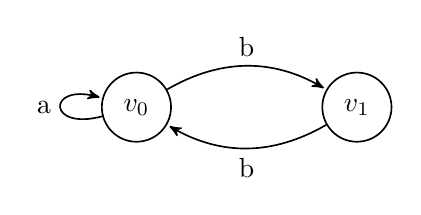
\begin{tikzpicture}[->,>=stealth',shorten >=1pt,auto,node distance=2.8cm, semithick]

    \node[state] (A)                    {$v_0$};
    \node[state]         (B) [right of=A] {$v_1$};
    
    \path (A) edge  [loop left] node {a} (A)
                edge  [bend left] node {b} (B)
            (B) edge  [bend left] node {b} (A);
    \end{tikzpicture}

    \caption{Input graph.}
    \label{fig:input-graph}

\end{figure}

\begin{figure}
    \centering
    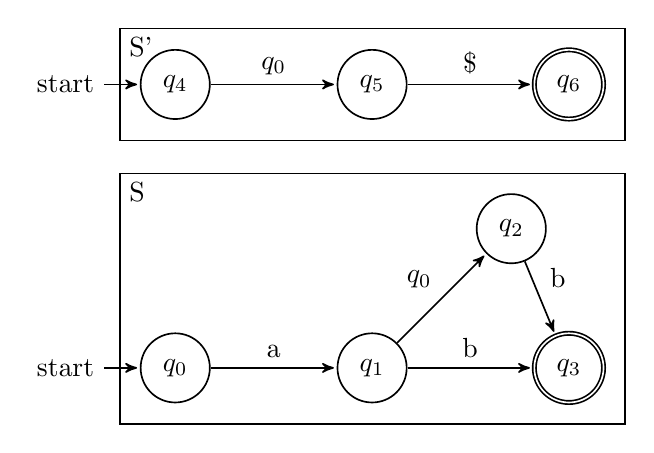
\begin{tikzpicture}[->,>=stealth',shorten >=1pt,auto,node distance=2.5cm, semithick]

    \node[initial,state]   (F)              {$q_4$};
    \node[state]           (G) [right of=F] {$q_5$};
    \node[accepting,state] (H) [right of=G] {$q_6$};
    \node[draw=black, fit= (F) (G) (H), inner sep=0.25cm] (J) {};
    \node[below right] at (J.north west) {S'};

    \path (F) edge              node {$q_0$} (G)
            (G) edge              node {$\$$} (H); 

    \node[initial,state] (A) [below = 2.7cm of F] {$q_0$};
    \node[state]         (B) [right of=A] {$q_1$};
    \node[state]         (D) [above right of=B] {$q_2$};
    \node[accepting,state]         (C) [right of=B] {$q_3$};
    \node [draw=black, fit= (A) (C) (D), inner sep=0.25cm] (E) {};
    \node[below right] at (E.north west) {S};

    \path (A) edge              node {a} (B)
            (B) edge              node {$q_0$} (D)
                edge              node {b} (C)
            (D) edge              node {b} (C);
    \end{tikzpicture}
    
    \caption{Extended RSM for grammar $S \to a \ b \mid a \ S \ b$. We automatically add the rule $S' \to S \ \$ $ to simplify query processing termination condition.}
    \label{fig:example-rsm}
\end{figure}

The resulting SPPF is shown in Fig.~\ref{fig:SPPF}.
Its root is the node $R^{q_4,v_0}_{q_5,v_0}$, which indicates that it represents paths from $v_0$ to $v_0$ that can be recognized by the RSM transitioning from state $q_4$ to $q_5$.
This transition corresponds to recognizing a word derived from the nonterminal $S$.
The node $R^{q_0,v_0}_{q_3,v_0}$ is the entry point for a cycle.
The node $R^{q_0,v_0}_{q_3,v_1}$ has two siblings, indicating two ways to construct the corresponding subpath.
The first corresponds to the shortest possible path: $$v_0 \xrightarrow{a} v_0 \xrightarrow{a} v_0 \xrightarrow{b} v_1 \xrightarrow{b} v_0.$$
The second contains the cycle mentioned above and therefore represents an infinite family of paths formed by repeatedly wrapping the shortest path with additional pairs of $a$s and $b$s.
For example, traversing the cycle once yields the path: $$v_0 \xrightarrow{a} v_0 \xrightarrow{a} v_0 \xrightarrow{a} v_0 \xrightarrow{a} v_0 \xrightarrow{b} v_1 \xrightarrow{b} v_0 \xrightarrow{b} v_1 \xrightarrow{b} v_0.$$

\input{texfigures/sppf}

\documentclass[
11pt,%
tightenlines,%
twoside,%
onecolumn,%
nobibnotes,%
nofootinbib,%
superscriptaddress,%
noshowpacs,%
centertags]%
{revtex4-2}
\usepackage{ljm}
\setcaptionwidth{0.93\textwidth}

% --- ГРАФИКА (WINDOWS) ---
\usepackage{epstopdf} % Критично для Windows: конвертирует EPS на лету
\graphicspath{{figures/}} 

% --- СТИЛЬ ЖУРНАЛА ---
\usepackage{ljm} % Файл должен лежать рядом!

% --- МАТЕМАТИКА И ТАБЛИЦЫ ---
\usepackage{mathtools}
\usepackage{colortbl}
\usepackage{algorithm2e}
% \usepackage{multirow}
\usepackage{makecell}  %new line in one table cell

% --- TIKZ (ВНИМАНИЕ: Для журнала в итоге нужны EPS файлы) ---
\usepackage{pgf}
\usepackage{tikz}
\usepackage{nicematrix}
\usetikzlibrary{arrows, automata, fit, calc, positioning}

% --- ДОПОЛНИТЕЛЬНО ---
% \usepackage{soul}
\usepackage[makeroom]{cancel}
\newcommand{\mycomment}[1]{}

\usepackage[caption=false]{subfig}
\usepackage{wrapfig}

\begin{document}
%
\title{GLL-based Context-Free Path Querying for Neo4j}

% --- АВТОРЫ (Формат RevTeX) ---

\author{Vadim Abzalov}
\email[E-mail: ]{vadim.i.abzalov@gmail.com}
\affiliation{Saint Petersburg State University, St. Petersburg, Russia}

\author{Vlada Pogozhelskaya}
\email[E-mail: ]{vvpogozhelskaia@edu.hse.ru}
\affiliation{National Research University Higher School of Economics, St. Petersburg, Russia}

\author{Vladimir Kutuev}
\email[E-mail: ]{v.kutuev@spbu.ru}
\affiliation{Saint Petersburg State University, St. Petersburg, Russia}

\author{Olga Bachishche}
\email[E-mail: ]{bachisheo@gmail.com}
\affiliation{ITMO University, St. Petersburg, Russia}

\author{Semyon Grigorev}
\email[E-mail: ]{s.v.grigoriev@spbu.ru}
\affiliation{Saint Petersburg State University, St. Petersburg, Russia}


% --- АННОТАЦИЯ (Должна быть ДО maketitle) ---
\begin{abstract}
We propose a GLL-based \textit{context-free path querying} algorithm that handles queries in Extended Backus-Naur Form (EBNF) using Recursive State Machines (RSM). Utilization of EBNF allows one to combine traditional regular expressions and mutually recursive patterns in constraints natively. The proposed algorithm solves both the \textit{reachability-only} and the \textit{all-paths} problems for the \textit{all-pairs} and the \textit{multiple sources} cases. The evaluation on real-world graphs demonstrates that the utilization of RSMs increases the performance of query evaluation. Being implemented as a stored procedure for Neo4j, our solution demonstrates better performance than a similar solution for RedisGraph. The performance of our solution on regular path queries is comparable to the performance of the native Neo4j solution, and in some cases, our solution requires significantly less memory.
\end{abstract}

% --- КЛЮЧЕВЫЕ СЛОВА ---
\keywords{Graph database, graph querying, context-free path querying, CFPQ, reachability problem, all-paths problem, generalized LL, GLL}

% --- ГЕНЕРАЦИЯ ЗАГОЛОВКА ---
\maketitle
\renewcommand{\figurename}{Fig.} 
% --- MAIN CONTENT ---
\input{sections/introduction}
\input{sections/preliminaries}
\input{sections/rsm}
\input{sections/gll}
\input{sections/dataset}
\input{sections/bnf_vs_ebnf}
\input{sections/cfpq_for_neo4j}
\input{sections/related_work}
\input{sections/conclusion}

\section*{ACKNOWLEDGMENTS}
We thank Adrian Johnstone for pointing out the Generalized LL algorithm in our discussion at Parsing@SLE--2013, which motivated the development of the presented solution. We thank George Fletcher for the discussion of the evaluation of different CFPQ algorithms for Neo4j.

\section*{FUNDING}
The study was funded by the St. Petersburg State University (Grant No. 116636233). 

\section*{CONFLICT OF INTEREST}
The authors of this work declare that they have no conflicts of interest.

%
% ---- Bibliography ----
%
% The bibliography style 'APS (American Physical Society)' is a standad for RevTex.
% References will then be sorted and formatted in the correct style.
%
\bibliographystyle{apsrev4-2}
\bibliography{gll}
%
\end{document}
\section{Experiment design}\label{section:dataset}
In this section, we provide a description of the graphs and queries used for the evaluation of the implemented algorithms. Also, we describe common evaluation scenarios and evaluation environment.

We evaluated our solution on both classical regular and context-free path queries to estimate the ability to use the proposed algorithm as a universal algorithm for the wide range of queries. 

\subsection{Graphs}

For the evaluation, we use a number of graphs from the CFPQ\_Data~\cite{cfpq-data} data set. We selected a number of graphs related to RDF analysis.
%, as well as a number of graphs extracted from the Linux sources which related to static code analysis problems.
A detailed description of the graphs, namely the number of the vertices and edges and the number of the edges labeled by tags used in the queries, is in Table~\ref{tab:graphs_for_evaluation_rdf}. Here ``bt'' is an abbreviation for \textit{broaderTransitive} relationship.

%) and in table~\ref{tab:graphs_for_evaluation_stat} for static code analysis. 

\begin{table}
    \caption{RDF graphs for evaluation: number of the vertices and edges, and number of the edges with specific label.}
    \label{tab:graphs_for_evaluation_rdf}
    \centering
    \scalebox{1}{
    \rowcolors{2}{black!2}{black!10}
    \begin{tabular}{| l | c | c | c | c | c | c |}
         \hline
         Graph name & $|V|$ & $|E|$ & \#subClassOf & \#type & \#bt\\
         \hline
         \hline
         Core               & 1 323     & 2 752      & 178        & 0        & 0 \\
         Pathways           & 6 238     & 12 363     & 3 117      & 3 118     & 0 \\
         Go\_hierarchy       & 45 007    & 490 109    & 490 109    & 0         & 0 \\
         Enzyme             & 48 815    & 86 543     & 8 163      & 14 989    & 8 156\\
         Eclass             & 239 111   & 360 248    & 90 962     & 72 517    & 0 \\
         Geospecies         & 450 609   & 2 201 532  & 0          & 89 065    & 20 867 \\
         Go                 & 582 929   & 1 437 437  & 94 514     & 226 481   & 0 \\
         Taxonomy           & 5 728 398 & 14 922 125 & 2 112 637  & 2 508 635 & 0 \\
         \hline
    \end{tabular}
    }
\end{table}
    
%\begin{table}[h!]
%    \centering
%    \rowcolors{2}{black!2}{black!10}
%    \begin{tabular}{| c | c | c | c | c | c | c |}
%         \hline
%         Graph name & $|V|$ & $|E|$ & \#a & \#d \\
%         \hline
%         \hline
%         Apache         & 1 721 418 & 1 510 411  & 362 799 & 1 147 612 \\
%         Block          & 3 423 234 & 2 951 393  & 669 238 & 2 282 155 \\
%         Fs             & 4 177 416 & 3 609 373 & 824 430 & 2 784 943 \\
%         Ipc            & 3 401 022 & 2 931 498 & 664 151 & 2 267 347 \\
%         Lib            & 3 401 355 & 2 931 880 & 664 311 & 2 267 569 \\
%         Mm             & 2 538 243 & 2 191 079 & 498 918 & 1 692 161 \\
%         Net            & 4 039 470 & 3 500 141 & 807 162 & 2 692 979 \\
%         Postgre        & 5 203 419 & 4 678 543 & 1 209 597 & 3 468 946 \\
%         Security       & 3 479 982 & 3 003 326 & 683 339 & 2 319 987 \\
%         Sound          & 3 528 861 & 3 049 732 & 697 159 & 2 352 573 \\
%         Init           & 2 446 224 & 2 112 809 & 481 994 & 1 630 815 \\
%         Arch           & 3 448 422 & 2 970 242 & 6 712 95 & 2 298 947 \\
%         Crypto         & 3 464 970 & 2 988 387 & 678 408 & 2 309 979 \\
%         Drivers        & 4 273 803 & 3 707 769 & 858 568 & 2 849 201 \\
%         Kernel         & 11 254 434& 9 484 213  & 1 981 258 & 7 502 955 \\
%         \hline
%    \end{tabular}
%    \caption{Points-to graphs for evaluation: number of vertices and edges, and number of edges with specific label}
%    \label{tab:graphs_for_evaluation_stat}
%\end{table}

To evaluate regular path queries, we used only RDF graphs, because code analysis graphs contain only two types of labels. Regular queries over such graphs are meaningless.

\subsection{Regular Queries}

Regular queries were generated using a well-established set of templates for RPQ algorithms evaluation. Namely, we use templates presented in Table 2 in~\cite{Pacaci2020RegularPQ} and in Table 5 in~\cite{Wang2019}. We select four non-trivial templates (that contain compositions of Kleene star and union) that are expressible in Cypher syntax to be able to compare the native Neo4j querying algorithm with our solution. Used templates are presented in equations~\ref{eqn:reg_1},~\ref{eqn:reg_2},~\ref{eqn:reg_3}, and~\ref{eqn:reg_4}. Respective path patterns expressed in Cypher are presented in equations~\ref{eqn:cypher_reg_1},~\ref{eqn:cypher_reg_2},~\ref{eqn:cypher_reg_3}, and~\ref{eqn:cypher_reg_4}. Note that while Cypher's power is limited, our solution can handle arbitrary RPQs. We generate one query for each template and each graph. The most frequent relations from the given graph were used as symbols in the query template.

\begin{minipage}{0.44\textwidth}
\begin{align}
\textit{reg}_1 = & (a \mid b)^* \label{eqn:reg_1}\\
\textit{reg}_2 = & a^* \cdot b^* \label{eqn:reg_2}
\end{align}
\end{minipage}
\begin{minipage}{0.44\textwidth}
\begin{align}
\textit{reg}_3 = & (a \mid b \mid c)^+ \label{eqn:reg_3}\\
\textit{reg}_4 = & (a \mid b)^+ \cdot (c \mid d)^+ \label{eqn:reg_4}
\end{align}
\end{minipage}

\begin{align}
\textit{reg}_1^{\text{N4j}} = & \texttt{()-[:a | :b]->\{0,\}()} \label{eqn:cypher_reg_1}\\
\textit{reg}_2^{\text{N4j}} = & \texttt{()-[:a]->\{0,\}()-[:b]->\{0,\}()} \label{eqn:cypher_reg_2}\\
\textit{reg}_3^{\text{N4j}} = & \texttt{()-[:a | :b | :c]->\{1,\}()} \label{eqn:cypher_reg_3}\\
\textit{reg}_4^{\text{N4j}} = & \texttt{()-[:a | :b]->\{1,\}()-[:c | :d]->\{1,\}()} \label{eqn:cypher_reg_4}
\end{align}

Also note that \textit{go\_hierarchy} graph is excluded from evaluation because it contains only one type of edge, so it is impossible to express meaningful queries over it. 

\mycomment{
\begin{table}
    \centering
{\small
\renewcommand{\arraystretch}{1.2}
\rowcolors{2}{black!2}{black!10}
\begin{tabular}{|c|c||c|c|}
\hline

Name & Query & Name & Query \\
\hline
\hline
$Q_1$   & $a^*$                               & $Q_9^5$    & $(a \mid b \mid c \mid d \mid e)^+$                     \\
$Q_2$   & $a\cdot b^*$                        & $Q_{10}^2$ & $(a \mid b) \cdot c^*$                                  \\
$Q_3$   & $a \cdot b^* \cdot c^*$             & $Q_{10}^3$ & $(a \mid b \mid c)  \cdot d^*$                          \\
$Q_4^2$ & $(a \mid b)^*$                      & $Q_{10}^4$ & $(a \mid b \mid c \mid d)  \cdot e^*$                   \\
$Q_4^3$ & $(a \mid b \mid c)^*$               & $Q_{10}^5$ & $(a \mid b \mid c \mid d \mid e)  \cdot f^*$            \\
$Q_4^4$ & $(a \mid b \mid c \mid d)^*$        & $Q_{10}^2$ & $a \cdot b$                                             \\
$Q_4^5$ & $(a \mid b \mid c \mid d \mid e)^*$ & $Q_{11}^3$ & $a \cdot b \cdot c$                                     \\
$Q_5$   & $a \cdot b^* \cdot c$               & $Q_{11}^4$ & $a \cdot b \cdot c \cdot d$                             \\
$Q_6$   & $a^* \cdot b^*$                     & $Q_{11}^5$ & $a \cdot b \cdot c \cdot d \cdot f$                     \\
$Q_7$   & $a \cdot b \cdot c^*$               & $Q_{12}$   & $(a \cdot b)^+ \mid  (c \cdot d)^+$                     \\
$Q_8$   & $a? \cdot b^*$                      & $Q_{13}$   & $(a \cdot(b \cdot c)^*)^+ \mid  (d \cdot f)^+$          \\
$Q_9^2$ & $(a \mid b)^+$                      & $Q_{14}$   & $(a \cdot b \cdot (c \cdot d)^*)^+  \cdot (e \mid f)^*$ \\
$Q_9^3$ & $(a \mid b \mid c)^+$               & $Q_{15}$   & $(a \mid b)^+ \cdot (c \mid d)^+$                       \\
$Q_9^4$ & $(a \mid b \mid c \mid d)^+$        & $Q_{16}$   & $a \cdot b \cdot (c \mid d \mid e)$                     \\
\hline
\end{tabular}
}
\caption{Queries templates for RPQ evaluation}
\label{tbl:queries_templates}
\end{table}
}

\subsection{Context-Free Queries}

All queries used in our evaluation are variants of the \textit{same-generation query}. For the \textit{RDF} graphs we use the same queries that were used for CFPQ algorithms evaluation in other works~\cite{Azimov:2018:CPQ:3210259.3210264,Kuijpers:2019:ESC:3335783.3335791}: $G_1$~(\ref{eqn:g_1}), $G_2$~(\ref{eqn:g_2}), and $Geo$~(\ref{eqn:geo}). The queries are expressed as context-free grammars where $S$ is a nonterminal, \textit{subClassOf, type, broaderTransitive, }$ \overline{\textit{subClassOf}}$, $\overline{\textit{type}}$, $\overline{\textit{broaderTransitive}}$ are terminals or the labels of the edges. We denote the inverse of an $x$ relation and the respective edge as $\overline{x}$.

\begin{align}
\label{eqn:g_2}
S \to \overline{\textit{subClassOf}} \ \ S \ \textit{subClasOf} \mid \textit{subClassOf}
\end{align}

\begin{align}
\begin{split}
\label{eqn:g_1}
S \to & \overline{\textit{subClassOf}} \ \ S \ \textit{subClasOf} \mid \overline{\textit{type}} \ \ S \ \textit{type}\\   & \mid \overline{\textit{subClassOf}} \ \ \textit{subClassOf} \mid \overline{\textit{type}} \ \textit{type}
\end{split}
\end{align}

\begin{align}
\begin{split}
\label{eqn:geo}
S \to & \textit{broaderTransitive} \ \  S \ \overline{\textit{broaderTransitive}} \\
      & \mid \textit{broaderTransitive} \ \  \overline{\textit{broaderTransitive}}
\end{split}
\end{align}

Respective RSMs are presented in Fig.~\ref{fig:rsm_queries}~a for $G_1$, Fig.~\ref{fig:rsm_queries}~b for $G_2$, and Fig.~\ref{fig:rsm_queries}~c for \textit{Geo}.

\input{texfigures/queries}


%For \textit{Points-to} graphs we use a \textit{PointsTo} query~(\ref{eqn:points_to}) which describes a points-to analysis~\cite{Zheng}.

%\begin{align}
%\begin{split}
%\label{eqn:points_to}
%M & \to \overline{d} \ V \ d \\
%V & \to (M? \ \overline{a})^* \ M? \ (a \ M?)^* 
%\end{split}
%\end{align}

\subsection{Scenarios Description}

We evaluate the proposed solution on the \textit{multiple sources reachability} scenario. We assume that the size of the starting set is significantly less than the number of the input graph vertices. This limitation looks reasonable in practical cases.
%We omit \textit{all-pairs all-paths} because it seems impractical: the detailed analysis is often required only for paths within a specific subgraph, not the entire graph. 

The starting sets for the multiple sources querying are generated from all vertices of a graph with a random permutation. We use chunks of size 1, 10, 100. For graphs with less than 10~000 vertices, all vertices were used for querying. For graphs with from 10~000 to 100~000 vertices, 10\% of vertices were considered starting ones. For the graphs with more than 100~000 vertices, only 1\% of vertices were considered. We use the same sets for all cases in all experiments to be able to compare results.

To check the correctness of our solution and to force the result stream, we compute the number of reachable pairs for each query.

\subsection{Evaluation Environment}

We ran all experiments on a PC with Ubuntu 20.04 installed. It has an Intel Core i7-6700 CPU, 3.4GHz, 4 threads (hyper-threading is turned off), and DDR4 64Gb RAM. We use OpenJDK 64-Bit Server VM Corretto-17.0.8.8.1 (build 17.0.8.1+8-LTS, mixed mode, sharing). JVM was configured to use 55Gb of heap memory: both \texttt{xms} and \texttt{xmx} are set to 55Gb. 

We use Neo4j 5.12.0. Almost all configurations of Neo4j are default. We only set  \texttt{memory\_transaction\_global\_max\_size} to \texttt{0}, which means unlimited memory usage per transaction.

As a competitor for our implementation, we use a linear algebra-based solution, integrated to RedisGraph by Arseniy Terekhov et al. and described in~\cite{DBLP:conf/edbt/TerekhovPAZG21} and we use the configuration described in it for RedisGraph evaluation in our work.

\section{Performance of GLL on Queries in BNF and EBNF}\label{section:BFN_or_RSM}

As discussed above, different CFG representations can be used to define the query. The basic one is BNF, the more expressive (but not more powerful) is EBNF. EBNF can also speed up query evaluation by replacing some recursion with Kleene star, reducing stack usage.
RSMs natively encode EBNF grammars and can be processed by GLL (Section ~\ref{section:RSM}).

We implemented and evaluated two versions of the GLL-based CFPQ algorithm~\cite{kotgll}: one operates with grammar in BNF, and another one operates with grammar in EBNF and utilizes RSM to represent it. Both versions were evaluated in reachability-only mode to estimate performance differences and to choose the best one to integrate with Neo4j. 

\subsection{Evaluation}\label{section:cfg_vs_rsm}

To assess the applicability of the proposed solution, we evaluate it on a number of real-world graphs and queries described in section~\ref{section:dataset}.
We evaluate \textit{reachability-only} query performance across varying start-set sizes to estimate the speedup of the RSM-based approach over the BNF-based one.
The experimental study was conducted as follows.   

\begin{itemize}
    \item For all graphs, queries, and start vertex sets, described in section~\ref{section:dataset}, we measure evaluation time for both versions.
    \item Average time for each start vertex set size was calculated. Thus, for each graph, query, and start vertex set size, we have an average time of respective query evaluation.
    \item Speedup as a ratio of BNF-based version evaluation time to RSM-based version evaluation time was calculated.
\end{itemize}


Results are shown in Fig.~\ref{fig:speedup}. In most cases, the RSM-based version outperforms the BNF-based one, with speedups typically below 2 times but reaching over 5 times in some settings (Fig.~\ref{fig:speedup} c: graph \textit{pathways}, grammar \textit{Geo}). The mean speedup across all graphs and grammars is 1.5, indicating that RSM-based GLL is faster on average.


\newcommand\speedImageW{0.34}
\newcommand\speedImageScale{1.111}


\begin{figure}[htbp]%
    \centering%
    \begin{minipage}{\speedImageW\textwidth} % 
        \centering % 
        \includegraphics[width=\speedImageScale\textwidth]{figures/g1_kotgll_result.eps}
        \small (a) 
    \end{minipage}%
    \begin{minipage}{\speedImageW\textwidth}%
        \centering%
        \includegraphics[width=\speedImageScale\textwidth]{figures/g2_kotgll_result.eps}
        \small (b) 
    \end{minipage}%
    \begin{minipage}{\speedImageW\textwidth}%
        \centering%
        \includegraphics[width=\speedImageScale\textwidth]{figures/geo_kotgll_result.eps}
        \small (c)
    \end{minipage}%
    \caption{Multiple-source CFPQ reachability speedup (RSM over CFG) on RDF graphs for (a)~$G_1$, (b)~$G_2$, and (c)~$Geo$ queries.}
    \label{fig:speedup}
\end{figure}
\section{CFPQ For Neo4j}\label{section:cfpq_for_neo4j}

This section details integrating GLL-based CFPQ into the Neo4j graph database. We use the RSM-based variant because our comparison (Section~\ref{section:cfg_vs_rsm}) shows it outperforms the BNF-based one.
Also, we provide results of the implemented solution evaluation which show that, first of all, the provided solution is faster than a similar linear algebra-based solution for RedisGraph. In addition, we show that on RPQs our solution is compatible with the Neo4j native one and in some cases evaluates queries successfully while the native solution fails with an \textit{OutOfMemory} exception.

\subsection{Implementation Details}

Neo4j stored procedure is a mechanism through which query language can be extended by writing custom code in Java in such a way that it can be called directly via Cypher. %The Java code need to be compiled into a \texttt{jar} file and to be put in the plugins directory of Neo4j root folder. 

We implemented a Neo4j stored procedure which solves the reachability problem for the given set of the start vertices and the given query. The procedure can be called as follows:
$\texttt{CALL}~\texttt{cfpq.gll.getReachabilities(nodes, q)}$
where \texttt{nodes} is a collection of start nodes, and \texttt{q} is a string representation (or description) of RSM specified over relation types. The procedure outputs a stream of reachable node pairs. Note that the expressive power of our solution is limited: we cannot use the full power of Cypher inside our constraints. For example, we cannot specify constraints on the vertices inside our constraints.

\mycomment{
%\scalebox{0.75}{\parbox{.5\linewidth}{%
\begin{align*}
StartState(&id=0,nonterminal=Nonterminal(S),\\
           &isStart=true,isFinal=false) \\
State(&id=1,nonterminal=Nonterminal(S), \\
      &isStart=false,isFinal=false) \\
State(&id=4,nonterminal=Nonterminal(S),isStart=false,isFinal=false) \\
State(&id=3,nonterminal=Nonterminal(S),isStart=false,isFinal=true) \\
State(&id=2,nonterminal=Nonterminal(S),isStart=false,isFinal=false) \\
State(&id=5,nonterminal=Nonterminal(S), \\
      &isStart=false,isFinal=false) \\
TerminalEdge(&tail=0,head=1,terminal=Terminal(subClassOf\_r)) \\
TerminalEdge(&tail=0,head=4,terminal=Terminal(type\_r)) \\
TerminalEdge(&tail=1,head=3,terminal=Terminal(subClassOf)) \\
NonterminalEdge(&tail=1,head=2,nonterminal=Nonterminal(S)) \\
TerminalEdge(&tail=4,head=3,terminal=Terminal(type)) \\
NonterminalEdge(&tail=4,head=5,nonterminal=Nonterminal(S)) \\
TerminalEdge(&tail=2,head=3,terminal=Terminal(subClassOf)) \\
TerminalEdge(&tail=5,head=3,terminal=Terminal(type))
\end{align*}
}
%}}
% \begin{figure}[ht]
%     \centering
%     \includegraphics[width=0.47\textwidth]{architecture.pdf}
%     \caption{Architecture of the solution}
%     \label{fig:solution_architecture}
% \end{figure}

We implemented a wrapper for Neo4j. Communication with the database is done using the Neo4j Native Java API. So, we used an embedded database, which means it is run inside of the application and is not used as an external service.

Along with the existing modifications of GLL, we made a Neo4j-specific one. Neo4j return result should be represented as a \texttt{Stream} and it is important to prevent early stream forcing, thus we changed all GLL internals to ensure that. This also has an added benefit that the query result is a stream, and thus it is possible to get the results on demand. 

\subsection{Evaluation}

To assess the applicability of the proposed solution, we evaluate it on a number of real-world graphs and queries. To estimate relative performance, we compare our solution with the matrix-based CFPQ algorithm implemented in RedisGraph by Arseniy Terekhov et al in~\cite{DBLP:conf/edbt/TerekhovPAZG21}. Also, we compare the performance of the query evaluation in \textit{reachability-only} mode on regular path queries with the native Neo4j solution.

%\subsection{Evaluation Results}

The results of the context-free path query evaluations are presented in Fig.~\ref{fig:performance}. 
Evaluation time depends not only on graph size and sparsity, but also on graph structure. 
For example, a relatively small graph \textit{go\_hierarchy} fully consists of edges used in queries $G_1$ and $G_2$, thus evaluation time for these queries is significantly bigger than for some bigger but more sparse graphs, for example, for the \textit{eclass} graph. Especially for a relatively large starting vertex set. Note that the creation of the relevant metrics for the CFPQ query evaluation time prediction is a challenging problem by itself and should be tackled in the future.

In almost all cases, the proposed solution is significantly faster than RedisGraph (in orders of magnitude in some cases).
In some cases, however (e.g., graph \textit{core} across all queries), RedisGraph outperforms our solution. Moreover, it can be seen that evaluation time for RedisGraph is more predictable. For our solution, in some cases, execution time highly depends on the start set. For example, see Fig.~\ref{fig:performance}~c, graph \textit{enzyme}.    

\newcommand\squeryImageW{0.34}
\newcommand\squeryImageScale{1.111}
\begin{figure}
    \begin{minipage}{\squeryImageW\textwidth}
        \centering
        \includegraphics[width=\squeryImageScale\textwidth]{figures/g1_result.eps}
        \small{(a)}
    \end{minipage}%
    \begin{minipage}{\squeryImageW\textwidth}
        \centering
    \includegraphics[width=\squeryImageScale\textwidth]{figures/g2_result.eps}
    \small{(b)}
    \end{minipage}%
    \begin{minipage}{\squeryImageW\textwidth}
        \centering
    \includegraphics[width=\squeryImageScale\textwidth]{figures/geo_result.eps}
    \small{(c)}
    \end{minipage}%
    \caption{Multiple source CFPQ reachability results for the queries: (a)~$G_1$, (b)~$G_2$, (c)~$Geo$ related to RDF analysis.}
    \label{fig:performance}
\end{figure}


The particularly important scenario is when the start set contains a single vertex. \texttt{Single-source reachability} queries are reasonably fast: median runtime is about few milliseconds across all graphs and queries. Even in this setting, runtime depends strongly on graph structure. For example, \textit{core} is slower than the other graphs despite being the smallest by node and edge count. Predicting execution time with a reliable metric remains non-trivial. As expected, runtime increases with chunk size.


Partial results for RPQ evaluation are presented in Fig.~\ref{fig:performance-reg}. For queries $\textit{reg}_3$ (defined in~\ref{eqn:reg_3}) and $\textit{reg}_4$ (defined in~\ref{eqn:reg_4}) we get similar results. Note that on \textit{geospecies} and \textit{taxonomy} graphs, the native solution failed with the \textit{OutOfMemory} exception, while our solution evaluates queries successfully. 

\begin{figure}
    \begin{minipage}{0.4\textwidth}
        \includegraphics[width=1.0125\textwidth]{figures/reg1_rpq_result.eps}
        \small{(a)}
    \end{minipage}%
    \begin{minipage}{0.4\textwidth}
        \includegraphics[width=1.0125\textwidth]{figures/reg2_rpq_result.eps}
        \small{(b)}
    \end{minipage}%   
    \centering
    \caption{Multiple source RPQ reachability results for queries related to RDF analysis: (a)~$\textit{reg}_1$ query, (b)~$\textit{reg}_2$ query (native solution failed with OOM on the last two graphs).}
    \label{fig:performance-reg}
\end{figure}


We can see that the proposed solution is slightly slower than the native Neo4j algorithm, but not dramatically: typically less than two times. Moreover, in some cases, our solution is comparable with the native one (see Fig.~\ref{fig:performance-reg}~a and Fig.~\ref{fig:performance-reg}~b, graph \textit{eclass}), and in some cases, our solution is faster than the native one (see Fig.~\ref{fig:performance-reg}~b, graph \textit{core}).

Finally, we conclude that the proposed GLL-based solution can serve as an alternative to linear algebra-based CFPQ algorithms and is suitable for real-world graph analysis systems: our evaluation shows that the proposed solution outperforms the linear algebra-based one. Furthermore, we show that the proposed solution can be used as a universal algorithm for both RPQ and CFPQ.
\section{Related Work}\label{section:related_work}

The idea to use context-free grammars as constraints in the path finding problem in the graph databases was introduced and explored by Mihalis Yannakakis in~\cite{10.1145/298514.298576}. Later, Thomas Reps et al. developed the same idea into a general framework for static code analysis~\cite{10.1145/199448.199462}.
This framework, called Context-Free Language Reachability (CFL-r), is widely used and actively studied. The landscape analysis of the area was recently provided by Andreas Pavlogiannis in~\cite{10.1145/3583660.3583664}. In the context of the graph databases, the most recent systematic comparison of different CFPQ algorithms was done by Jochem Kuijpers et al. A set of CFPQ algorithms was implemented and evaluated using Neo4j as a graph storage. Results were presented in~\cite{Kuijpers:2019:ESC:3335783.3335791}. It was concluded that the existing algorithms are not performant enough to be used for the real-world data analysis.

Regarding graph databases, CFPQ was applied in such graph analysis related tasks as biological data analysis~\cite{SubgraphQueriesbyContextfreeGrammars}, data provenance~\cite{8731467}, hierarchy analysis in RDF data~\cite{MEDEIROS2022101089,zhangCfPgRdf}.

Multiple CFPQ algorithms are based on different parsing algorithms and techniques. For example, an approach based on parsing combinators was proposed by Ekaterina Verbitskaia et al. in~\cite{10.1145/3241653.3241655}. Several algorithms based on LL-like and LR-like techniques were developed by Ciro M. Medeiros et al. in~\cite{10.1145/3427081.3427087,MEDEIROS201975,MEDEIROS2022101089}. Also, CFPQ algorithms were investigated by Phillip Bradford in~\cite{Bradford2009,8249039} and Charles B. Ward et al. in~\cite{4625871}. An algorithm based on matrix equations was proposed by Yuliya Susanina in~\cite{10.1145/3318464.3384400}.
Paths extraction problem was studied by Jelle Hellings in~\cite{Hellings2020ExplainingPQ}.

A set of linear-algebra-based CFPQ algorithms was developed by Rustam Azimov et al., including all-path and single-path variants, proposed in~\cite{10.1145/3461837.3464513} and~\cite{10.1145/3398682.3399163}, respectively. The Kronecker product-based algorithm~\cite{OrachevKronecker} was proposed by Egor Orachev et al., and a multiple-source CFPQ algorithm for RedisGraph was proposed by Arseniy Terekhov et al. in~\cite{DBLP:conf/edbt/TerekhovPAZG21}. 

Recursive state machines were studied in the context of CFPQ in several papers, including~\cite{OrachevKronecker} where Egor Orachev et al. use RSM to specify context-free constraints, Yuxiang Lei et al.~\cite{10.1145/3591233} propose to use RSM to specify path constraints, and~\cite{10.1145/1328438.1328460} where Swarat Chaudhuri proposes a slightly subcubic algorithm for the reachability problem for recursive state machines --- the equivalent to CFPQ problem.

GLL was introduced by Elizabeth Scott and Adrian Johnstone in~\cite{SCOTT2010177}. A number of modifications of the GLL algorithm were further proposed, including the version which supports EBNF without its transformation~\cite{SCOTT2018120} and the version which uses binary subtree sets~\cite{SCOTT201963} instead of SPPF. The latest version simplifies the algorithm and avoids the overhead of the explicit graph construction. Within it, the optimized and simplified OOP-friendly version of GLL was proposed by Ali Afroozeh and Anastasia Izmaylova in~\cite{AfroozenFasterGll}.
\section{Conclusion and Future Work}\label{section:conclusion}

In this work, we presented the GLL-based context-free path querying algorithm for the Neo4j graph database. The implementation is available on GitHub: \url{https://github.com/vadyushkins/cfpq-gll-neo4j-procedure}.

Our solution uses Neo4j for graph storage, but the query language should be extended to support context-free constraints to make it useful. Both the extension of Cypher and the integration of our algorithm with the query engine are non-trivial challenges left for future work.

While GLL-based CFPQ can potentially be used to solve the \textit{all-paths} problem, currently we have implemented the procedure only for the reachability. The choice of effective strategies to enumerate paths and implementation of them is a direction for future research.  

The most important direction for future work is to find a way to provide an incremental version of the GLL-based CFPQ algorithm to avoid full query reevaluation when the graph is only slightly changed. While our solution is based on the well-known parsing algorithm and there are solutions for incremental parsing, development of the efficient incremental version of the GLL-based CFPQ algorithm is a challenging problem left for future research. 

Another direction is to create a parallel version of the GLL-based CFPQ algorithm to improve its performance on huge graphs. Although it seems natural to handle descriptors in parallel, the algorithm operates over global structures, and the na{\"{\i}}ve implementation of this idea leads to a significant overhead in synchronization.

\section*{ACKNOWLEDGMENTS}
We thank Adrian Johnstone for pointing out the Generalized LL algorithm in our discussion at Parsing@SLE--2013, which motivated the development of the presented solution. We thank George Fletcher for the discussion of the evaluation of different CFPQ algorithms for Neo4j.

\section*{FUNDING}
The study was funded by the St. Petersburg State University (Grant No. 116636233). 

\section*{CONFLICT OF INTEREST}
The authors of this work declare that they have no conflicts of interest.

%
% ---- Bibliography ----
%
% The bibliography style 'APS (American Physical Society)' is a standad for RevTex.
% References will then be sorted and formatted in the correct style.
%
\bibliographystyle{apsrev4-2}
\bibliography{gll}
%
\end{document}
\section{Experiment design}\label{section:dataset}
In this section, we provide a description of the graphs and queries used for the evaluation of the implemented algorithms. Also, we describe common evaluation scenarios and evaluation environment.

We evaluated our solution on both classical regular and context-free path queries to estimate the ability to use the proposed algorithm as a universal algorithm for the wide range of queries. 

\subsection{Graphs}

For the evaluation, we use a number of graphs from the CFPQ\_Data~\cite{cfpq-data} data set. We selected a number of graphs related to RDF analysis.
%, as well as a number of graphs extracted from the Linux sources which related to static code analysis problems.
A detailed description of the graphs, namely the number of the vertices and edges and the number of the edges labeled by tags used in the queries, is in Table~\ref{tab:graphs_for_evaluation_rdf}. Here ``bt'' is an abbreviation for \textit{broaderTransitive} relationship.

%) and in table~\ref{tab:graphs_for_evaluation_stat} for static code analysis. 

\begin{table}
    \caption{RDF graphs for evaluation: number of the vertices and edges, and number of the edges with specific label.}
    \label{tab:graphs_for_evaluation_rdf}
    \centering
    \scalebox{1}{
    \rowcolors{2}{black!2}{black!10}
    \begin{tabular}{| l | c | c | c | c | c | c |}
         \hline
         Graph name & $|V|$ & $|E|$ & \#subClassOf & \#type & \#bt\\
         \hline
         \hline
         Core               & 1 323     & 2 752      & 178        & 0        & 0 \\
         Pathways           & 6 238     & 12 363     & 3 117      & 3 118     & 0 \\
         Go\_hierarchy       & 45 007    & 490 109    & 490 109    & 0         & 0 \\
         Enzyme             & 48 815    & 86 543     & 8 163      & 14 989    & 8 156\\
         Eclass             & 239 111   & 360 248    & 90 962     & 72 517    & 0 \\
         Geospecies         & 450 609   & 2 201 532  & 0          & 89 065    & 20 867 \\
         Go                 & 582 929   & 1 437 437  & 94 514     & 226 481   & 0 \\
         Taxonomy           & 5 728 398 & 14 922 125 & 2 112 637  & 2 508 635 & 0 \\
         \hline
    \end{tabular}
    }
\end{table}
    
%\begin{table}[h!]
%    \centering
%    \rowcolors{2}{black!2}{black!10}
%    \begin{tabular}{| c | c | c | c | c | c | c |}
%         \hline
%         Graph name & $|V|$ & $|E|$ & \#a & \#d \\
%         \hline
%         \hline
%         Apache         & 1 721 418 & 1 510 411  & 362 799 & 1 147 612 \\
%         Block          & 3 423 234 & 2 951 393  & 669 238 & 2 282 155 \\
%         Fs             & 4 177 416 & 3 609 373 & 824 430 & 2 784 943 \\
%         Ipc            & 3 401 022 & 2 931 498 & 664 151 & 2 267 347 \\
%         Lib            & 3 401 355 & 2 931 880 & 664 311 & 2 267 569 \\
%         Mm             & 2 538 243 & 2 191 079 & 498 918 & 1 692 161 \\
%         Net            & 4 039 470 & 3 500 141 & 807 162 & 2 692 979 \\
%         Postgre        & 5 203 419 & 4 678 543 & 1 209 597 & 3 468 946 \\
%         Security       & 3 479 982 & 3 003 326 & 683 339 & 2 319 987 \\
%         Sound          & 3 528 861 & 3 049 732 & 697 159 & 2 352 573 \\
%         Init           & 2 446 224 & 2 112 809 & 481 994 & 1 630 815 \\
%         Arch           & 3 448 422 & 2 970 242 & 6 712 95 & 2 298 947 \\
%         Crypto         & 3 464 970 & 2 988 387 & 678 408 & 2 309 979 \\
%         Drivers        & 4 273 803 & 3 707 769 & 858 568 & 2 849 201 \\
%         Kernel         & 11 254 434& 9 484 213  & 1 981 258 & 7 502 955 \\
%         \hline
%    \end{tabular}
%    \caption{Points-to graphs for evaluation: number of vertices and edges, and number of edges with specific label}
%    \label{tab:graphs_for_evaluation_stat}
%\end{table}

To evaluate regular path queries, we used only RDF graphs, because code analysis graphs contain only two types of labels. Regular queries over such graphs are meaningless.

\subsection{Regular Queries}

Regular queries were generated using a well-established set of templates for RPQ algorithms evaluation. Namely, we use templates presented in Table 2 in~\cite{Pacaci2020RegularPQ} and in Table 5 in~\cite{Wang2019}. We select four non-trivial templates (that contain compositions of Kleene star and union) that are expressible in Cypher syntax to be able to compare the native Neo4j querying algorithm with our solution. Used templates are presented in equations~\ref{eqn:reg_1},~\ref{eqn:reg_2},~\ref{eqn:reg_3}, and~\ref{eqn:reg_4}. Respective path patterns expressed in Cypher are presented in equations~\ref{eqn:cypher_reg_1},~\ref{eqn:cypher_reg_2},~\ref{eqn:cypher_reg_3}, and~\ref{eqn:cypher_reg_4}. Note that while Cypher's power is limited, our solution can handle arbitrary RPQs. We generate one query for each template and each graph. The most frequent relations from the given graph were used as symbols in the query template.

\begin{minipage}{0.44\textwidth}
\begin{align}
\textit{reg}_1 = & (a \mid b)^* \label{eqn:reg_1}\\
\textit{reg}_2 = & a^* \cdot b^* \label{eqn:reg_2}
\end{align}
\end{minipage}
\begin{minipage}{0.44\textwidth}
\begin{align}
\textit{reg}_3 = & (a \mid b \mid c)^+ \label{eqn:reg_3}\\
\textit{reg}_4 = & (a \mid b)^+ \cdot (c \mid d)^+ \label{eqn:reg_4}
\end{align}
\end{minipage}

\begin{align}
\textit{reg}_1^{\text{N4j}} = & \texttt{()-[:a | :b]->\{0,\}()} \label{eqn:cypher_reg_1}\\
\textit{reg}_2^{\text{N4j}} = & \texttt{()-[:a]->\{0,\}()-[:b]->\{0,\}()} \label{eqn:cypher_reg_2}\\
\textit{reg}_3^{\text{N4j}} = & \texttt{()-[:a | :b | :c]->\{1,\}()} \label{eqn:cypher_reg_3}\\
\textit{reg}_4^{\text{N4j}} = & \texttt{()-[:a | :b]->\{1,\}()-[:c | :d]->\{1,\}()} \label{eqn:cypher_reg_4}
\end{align}

Also note that \textit{go\_hierarchy} graph is excluded from evaluation because it contains only one type of edge, so it is impossible to express meaningful queries over it. 

\mycomment{
\begin{table}
    \centering
{\small
\renewcommand{\arraystretch}{1.2}
\rowcolors{2}{black!2}{black!10}
\begin{tabular}{|c|c||c|c|}
\hline

Name & Query & Name & Query \\
\hline
\hline
$Q_1$   & $a^*$                               & $Q_9^5$    & $(a \mid b \mid c \mid d \mid e)^+$                     \\
$Q_2$   & $a\cdot b^*$                        & $Q_{10}^2$ & $(a \mid b) \cdot c^*$                                  \\
$Q_3$   & $a \cdot b^* \cdot c^*$             & $Q_{10}^3$ & $(a \mid b \mid c)  \cdot d^*$                          \\
$Q_4^2$ & $(a \mid b)^*$                      & $Q_{10}^4$ & $(a \mid b \mid c \mid d)  \cdot e^*$                   \\
$Q_4^3$ & $(a \mid b \mid c)^*$               & $Q_{10}^5$ & $(a \mid b \mid c \mid d \mid e)  \cdot f^*$            \\
$Q_4^4$ & $(a \mid b \mid c \mid d)^*$        & $Q_{10}^2$ & $a \cdot b$                                             \\
$Q_4^5$ & $(a \mid b \mid c \mid d \mid e)^*$ & $Q_{11}^3$ & $a \cdot b \cdot c$                                     \\
$Q_5$   & $a \cdot b^* \cdot c$               & $Q_{11}^4$ & $a \cdot b \cdot c \cdot d$                             \\
$Q_6$   & $a^* \cdot b^*$                     & $Q_{11}^5$ & $a \cdot b \cdot c \cdot d \cdot f$                     \\
$Q_7$   & $a \cdot b \cdot c^*$               & $Q_{12}$   & $(a \cdot b)^+ \mid  (c \cdot d)^+$                     \\
$Q_8$   & $a? \cdot b^*$                      & $Q_{13}$   & $(a \cdot(b \cdot c)^*)^+ \mid  (d \cdot f)^+$          \\
$Q_9^2$ & $(a \mid b)^+$                      & $Q_{14}$   & $(a \cdot b \cdot (c \cdot d)^*)^+  \cdot (e \mid f)^*$ \\
$Q_9^3$ & $(a \mid b \mid c)^+$               & $Q_{15}$   & $(a \mid b)^+ \cdot (c \mid d)^+$                       \\
$Q_9^4$ & $(a \mid b \mid c \mid d)^+$        & $Q_{16}$   & $a \cdot b \cdot (c \mid d \mid e)$                     \\
\hline
\end{tabular}
}
\caption{Queries templates for RPQ evaluation}
\label{tbl:queries_templates}
\end{table}
}

\subsection{Context-Free Queries}

All queries used in our evaluation are variants of the \textit{same-generation query}. For the \textit{RDF} graphs we use the same queries that were used for CFPQ algorithms evaluation in other works~\cite{Azimov:2018:CPQ:3210259.3210264,Kuijpers:2019:ESC:3335783.3335791}: $G_1$~(\ref{eqn:g_1}), $G_2$~(\ref{eqn:g_2}), and $Geo$~(\ref{eqn:geo}). The queries are expressed as context-free grammars where $S$ is a nonterminal, \textit{subClassOf, type, broaderTransitive, }$ \overline{\textit{subClassOf}}$, $\overline{\textit{type}}$, $\overline{\textit{broaderTransitive}}$ are terminals or the labels of the edges. We denote the inverse of an $x$ relation and the respective edge as $\overline{x}$.

\begin{align}
\label{eqn:g_2}
S \to \overline{\textit{subClassOf}} \ \ S \ \textit{subClasOf} \mid \textit{subClassOf}
\end{align}

\begin{align}
\begin{split}
\label{eqn:g_1}
S \to & \overline{\textit{subClassOf}} \ \ S \ \textit{subClasOf} \mid \overline{\textit{type}} \ \ S \ \textit{type}\\   & \mid \overline{\textit{subClassOf}} \ \ \textit{subClassOf} \mid \overline{\textit{type}} \ \textit{type}
\end{split}
\end{align}

\begin{align}
\begin{split}
\label{eqn:geo}
S \to & \textit{broaderTransitive} \ \  S \ \overline{\textit{broaderTransitive}} \\
      & \mid \textit{broaderTransitive} \ \  \overline{\textit{broaderTransitive}}
\end{split}
\end{align}

Respective RSMs are presented in Fig.~\ref{fig:rsm_queries}~a for $G_1$, Fig.~\ref{fig:rsm_queries}~b for $G_2$, and Fig.~\ref{fig:rsm_queries}~c for \textit{Geo}.

\newcommand{\nodeDistanceRsm}{2cm}
\newcommand{\rsmInnerXSep}{0.1cm}
\newcommand{\rsmInnerYSep}{0.8cm}

% ЛЕВАЯ (G1)
\newcommand{\rsmgone}[1][1.0]{%
\begin{tikzpicture}[thick,scale=#1, node distance=\nodeDistanceRsm,
                    shorten >=1pt,on grid,auto] 

  \node[state, initial above] (q_0)   {$q_0$};
  \node[state] (q_1) [below right=of q_0] {$q_1$};
  \node[state] (q_2) [below=of q_1] {$q_2$};
  \node[state, accepting] (q_3) [below left=of q_2] {$q_3$};
  \node[state] (q_4) [below left=of q_0] {$q_4$};
  \node[state] (q_5) [below=of q_4] {$q_5$};

  \node[draw=black, fit=(q_0) (q_1) (q_5) (q_3), inner xsep=0.1cm, inner ysep=0.1cm] (E) {};
  \node[below right] at (E.north west) {S};

  \path[->]
    (q_0) edge[sloped, right, above, bend left] node {$\overline{subClassOf}$} (q_1)
    (q_1) edge node {$q_0$} (q_2)
    (q_2) edge[sloped, right, below, bend left] node {$subClassOf$} (q_3)
    (q_1) edge[sloped, above] node {$subClassOf$} (q_3)
    (q_0) edge[bend right, sloped, below] node {$\overline{type}$} (q_4)
    (q_4) edge[left] node {$q_0$} (q_5)
    (q_5) edge[left, sloped, bend right, below] node {$type$} (q_3)
    (q_4) edge[sloped, above] node {$type$} (q_3);
\end{tikzpicture}%
}


% ПРАВАЯ ВЕРХНЯЯ (G2)
\newcommand{\rsmgtwo}[1][1.0]{%
\begin{tikzpicture}[thick,scale=#1, node distance=2cm,
                    shorten >=1pt,on grid,auto]
  \node[state, initial] (q_0)   {$q_0$};
  \node[state] (q_1) [right=of q_0] {$q_1$};
  \node[state] (q_2) [right=of q_1] {$q_2$};
  \node[state, accepting] (q_3) [right=of q_2] {$q_3$};
  \node[draw=black, fit=(q_0) (q_1) (q_3),
        inner xsep=\rsmInnerXSep, inner ysep=\rsmInnerYSep] (E) {};
  \node[below right] at (E.north west) {S};
  \path[->]
    (q_0) edge[bend right, below] node {$\overline{subClassOf}$} (q_1)
    (q_1) edge node {$q_0$} (q_2)
    (q_2) edge[bend right, below] node {$subClassOf$} (q_3)
    (q_0) edge[bend left, below]  node {$subClassOf$} (q_3);
\end{tikzpicture}%
}

% ПРАВАЯ НИЖНЯЯ (Geo)
\newcommand{\rsmgeo}[1][1.0]{%
\begin{tikzpicture}[thick,scale=#1, node distance=2cm,
                    shorten >=1pt,on grid,auto]
  \node[state, initial] (q_0)   {$q_0$};
  \node[state] (q_1) [right=of q_0] {$q_1$};
  \node[state] (q_2) [right=of q_1] {$q_2$};
  \node[state, accepting] (q_3) [right=of q_2] {$q_3$};
  \node[draw=black, fit=(q_0) (q_1) (q_3),
        inner xsep=\rsmInnerXSep, inner ysep=\rsmInnerYSep] (E) {};
  \node[below right] at (E.north west) {S};
  \path[->]
    (q_0) edge[bend left, above]  node {$broaderTransitive$} (q_1)
    (q_1) edge  node {$q_0$} (q_2)
    (q_2) edge[bend right, below] node {$\overline{broaderTransitive}$} (q_3)
    (q_1) edge[bend left, above]  node {$\overline{broaderTransitive}$} (q_3);
\end{tikzpicture}%
}


\begin{figure}[]
  \resizebox{0.8\textwidth}{!}{
      \begin{minipage}{0.4\textwidth}\vspace{0pt}
          \rsmgone[0.95]
          \small \\ (a)
      \end{minipage}\hspace{0pt}
      \begin{minipage}{0.53\textwidth}\vspace{0pt}
          \vspace{1.8em}
          \rsmgtwo[0.80]
          \small \\ (b)
        \vspace{1.4em}
    
          \rsmgeo[0.80]
          \small \\ (c)
      \end{minipage}
  }
  \caption{RSMs for queries: (a)~$G_1$~(\ref{eqn:g_1}), (b)~$G_2$~(\ref{eqn:g_2}), and (c)~$Geo$~(\ref{eqn:geo}).}
  \label{fig:rsm_queries}
\end{figure}



%For \textit{Points-to} graphs we use a \textit{PointsTo} query~(\ref{eqn:points_to}) which describes a points-to analysis~\cite{Zheng}.

%\begin{align}
%\begin{split}
%\label{eqn:points_to}
%M & \to \overline{d} \ V \ d \\
%V & \to (M? \ \overline{a})^* \ M? \ (a \ M?)^* 
%\end{split}
%\end{align}

\subsection{Scenarios Description}

We evaluate the proposed solution on the \textit{multiple sources reachability} scenario. We assume that the size of the starting set is significantly less than the number of the input graph vertices. This limitation looks reasonable in practical cases.
%We omit \textit{all-pairs all-paths} because it seems impractical: the detailed analysis is often required only for paths within a specific subgraph, not the entire graph. 

The starting sets for the multiple sources querying are generated from all vertices of a graph with a random permutation. We use chunks of size 1, 10, 100. For graphs with less than 10~000 vertices, all vertices were used for querying. For graphs with from 10~000 to 100~000 vertices, 10\% of vertices were considered starting ones. For the graphs with more than 100~000 vertices, only 1\% of vertices were considered. We use the same sets for all cases in all experiments to be able to compare results.

To check the correctness of our solution and to force the result stream, we compute the number of reachable pairs for each query.

\subsection{Evaluation Environment}

We ran all experiments on a PC with Ubuntu 20.04 installed. It has an Intel Core i7-6700 CPU, 3.4GHz, 4 threads (hyper-threading is turned off), and DDR4 64Gb RAM. We use OpenJDK 64-Bit Server VM Corretto-17.0.8.8.1 (build 17.0.8.1+8-LTS, mixed mode, sharing). JVM was configured to use 55Gb of heap memory: both \texttt{xms} and \texttt{xmx} are set to 55Gb. 

We use Neo4j 5.12.0. Almost all configurations of Neo4j are default. We only set  \texttt{memory\_transaction\_global\_max\_size} to \texttt{0}, which means unlimited memory usage per transaction.

As a competitor for our implementation, we use a linear algebra-based solution, integrated to RedisGraph by Arseniy Terekhov et al. and described in~\cite{DBLP:conf/edbt/TerekhovPAZG21} and we use the configuration described in it for RedisGraph evaluation in our work.

\section{Performance of GLL on Queries in BNF and EBNF}\label{section:BFN_or_RSM}

As discussed above, different CFG representations can be used to define the query. The basic one is BNF, the more expressive (but not more powerful) is EBNF. EBNF can also speed up query evaluation by replacing some recursion with Kleene star, reducing stack usage.
RSMs natively encode EBNF grammars and can be processed by GLL (Section ~\ref{section:RSM}).

We implemented and evaluated two versions of the GLL-based CFPQ algorithm~\cite{kotgll}: one operates with grammar in BNF, and another one operates with grammar in EBNF and utilizes RSM to represent it. Both versions were evaluated in reachability-only mode to estimate performance differences and to choose the best one to integrate with Neo4j. 

\subsection{Evaluation}\label{section:cfg_vs_rsm}

To assess the applicability of the proposed solution, we evaluate it on a number of real-world graphs and queries described in section~\ref{section:dataset}.
We evaluate \textit{reachability-only} query performance across varying start-set sizes to estimate the speedup of the RSM-based approach over the BNF-based one.
The experimental study was conducted as follows.   

\begin{itemize}
    \item For all graphs, queries, and start vertex sets, described in section~\ref{section:dataset}, we measure evaluation time for both versions.
    \item Average time for each start vertex set size was calculated. Thus, for each graph, query, and start vertex set size, we have an average time of respective query evaluation.
    \item Speedup as a ratio of BNF-based version evaluation time to RSM-based version evaluation time was calculated.
\end{itemize}


Results are shown in Fig.~\ref{fig:speedup}. In most cases, the RSM-based version outperforms the BNF-based one, with speedups typically below 2 times but reaching over 5 times in some settings (Fig.~\ref{fig:speedup} c: graph \textit{pathways}, grammar \textit{Geo}). The mean speedup across all graphs and grammars is 1.5, indicating that RSM-based GLL is faster on average.


\newcommand\speedImageW{0.34}
\newcommand\speedImageScale{1.111}


\begin{figure}[htbp]%
    \centering%
    \begin{minipage}{\speedImageW\textwidth} % 
        \centering % 
        \includegraphics[width=\speedImageScale\textwidth]{figures/g1_kotgll_result.eps}
        \small (a) 
    \end{minipage}%
    \begin{minipage}{\speedImageW\textwidth}%
        \centering%
        \includegraphics[width=\speedImageScale\textwidth]{figures/g2_kotgll_result.eps}
        \small (b) 
    \end{minipage}%
    \begin{minipage}{\speedImageW\textwidth}%
        \centering%
        \includegraphics[width=\speedImageScale\textwidth]{figures/geo_kotgll_result.eps}
        \small (c)
    \end{minipage}%
    \caption{Multiple-source CFPQ reachability speedup (RSM over CFG) on RDF graphs for (a)~$G_1$, (b)~$G_2$, and (c)~$Geo$ queries.}
    \label{fig:speedup}
\end{figure}
\section{CFPQ For Neo4j}\label{section:cfpq_for_neo4j}

This section details integrating GLL-based CFPQ into the Neo4j graph database. We use the RSM-based variant because our comparison (Section~\ref{section:cfg_vs_rsm}) shows it outperforms the BNF-based one.
Also, we provide results of the implemented solution evaluation which show that, first of all, the provided solution is faster than a similar linear algebra-based solution for RedisGraph. In addition, we show that on RPQs our solution is compatible with the Neo4j native one and in some cases evaluates queries successfully while the native solution fails with an \textit{OutOfMemory} exception.

\subsection{Implementation Details}

Neo4j stored procedure is a mechanism through which query language can be extended by writing custom code in Java in such a way that it can be called directly via Cypher. %The Java code need to be compiled into a \texttt{jar} file and to be put in the plugins directory of Neo4j root folder. 

We implemented a Neo4j stored procedure which solves the reachability problem for the given set of the start vertices and the given query. The procedure can be called as follows:
$\texttt{CALL}~\texttt{cfpq.gll.getReachabilities(nodes, q)}$
where \texttt{nodes} is a collection of start nodes, and \texttt{q} is a string representation (or description) of RSM specified over relation types. The procedure outputs a stream of reachable node pairs. Note that the expressive power of our solution is limited: we cannot use the full power of Cypher inside our constraints. For example, we cannot specify constraints on the vertices inside our constraints.

\mycomment{
%\scalebox{0.75}{\parbox{.5\linewidth}{%
\begin{align*}
StartState(&id=0,nonterminal=Nonterminal(S),\\
           &isStart=true,isFinal=false) \\
State(&id=1,nonterminal=Nonterminal(S), \\
      &isStart=false,isFinal=false) \\
State(&id=4,nonterminal=Nonterminal(S),isStart=false,isFinal=false) \\
State(&id=3,nonterminal=Nonterminal(S),isStart=false,isFinal=true) \\
State(&id=2,nonterminal=Nonterminal(S),isStart=false,isFinal=false) \\
State(&id=5,nonterminal=Nonterminal(S), \\
      &isStart=false,isFinal=false) \\
TerminalEdge(&tail=0,head=1,terminal=Terminal(subClassOf\_r)) \\
TerminalEdge(&tail=0,head=4,terminal=Terminal(type\_r)) \\
TerminalEdge(&tail=1,head=3,terminal=Terminal(subClassOf)) \\
NonterminalEdge(&tail=1,head=2,nonterminal=Nonterminal(S)) \\
TerminalEdge(&tail=4,head=3,terminal=Terminal(type)) \\
NonterminalEdge(&tail=4,head=5,nonterminal=Nonterminal(S)) \\
TerminalEdge(&tail=2,head=3,terminal=Terminal(subClassOf)) \\
TerminalEdge(&tail=5,head=3,terminal=Terminal(type))
\end{align*}
}
%}}
% \begin{figure}[ht]
%     \centering
%     \includegraphics[width=0.47\textwidth]{architecture.pdf}
%     \caption{Architecture of the solution}
%     \label{fig:solution_architecture}
% \end{figure}

We implemented a wrapper for Neo4j. Communication with the database is done using the Neo4j Native Java API. So, we used an embedded database, which means it is run inside of the application and is not used as an external service.

Along with the existing modifications of GLL, we made a Neo4j-specific one. Neo4j return result should be represented as a \texttt{Stream} and it is important to prevent early stream forcing, thus we changed all GLL internals to ensure that. This also has an added benefit that the query result is a stream, and thus it is possible to get the results on demand. 

\subsection{Evaluation}

To assess the applicability of the proposed solution, we evaluate it on a number of real-world graphs and queries. To estimate relative performance, we compare our solution with the matrix-based CFPQ algorithm implemented in RedisGraph by Arseniy Terekhov et al in~\cite{DBLP:conf/edbt/TerekhovPAZG21}. Also, we compare the performance of the query evaluation in \textit{reachability-only} mode on regular path queries with the native Neo4j solution.

%\subsection{Evaluation Results}

The results of the context-free path query evaluations are presented in Fig.~\ref{fig:performance}. 
Evaluation time depends not only on graph size and sparsity, but also on graph structure. 
For example, a relatively small graph \textit{go\_hierarchy} fully consists of edges used in queries $G_1$ and $G_2$, thus evaluation time for these queries is significantly bigger than for some bigger but more sparse graphs, for example, for the \textit{eclass} graph. Especially for a relatively large starting vertex set. Note that the creation of the relevant metrics for the CFPQ query evaluation time prediction is a challenging problem by itself and should be tackled in the future.

In almost all cases, the proposed solution is significantly faster than RedisGraph (in orders of magnitude in some cases).
In some cases, however (e.g., graph \textit{core} across all queries), RedisGraph outperforms our solution. Moreover, it can be seen that evaluation time for RedisGraph is more predictable. For our solution, in some cases, execution time highly depends on the start set. For example, see Fig.~\ref{fig:performance}~c, graph \textit{enzyme}.    

\newcommand\squeryImageW{0.34}
\newcommand\squeryImageScale{1.111}
\begin{figure}
    \begin{minipage}{\squeryImageW\textwidth}
        \centering
        \includegraphics[width=\squeryImageScale\textwidth]{figures/g1_result.eps}
        \small{(a)}
    \end{minipage}%
    \begin{minipage}{\squeryImageW\textwidth}
        \centering
    \includegraphics[width=\squeryImageScale\textwidth]{figures/g2_result.eps}
    \small{(b)}
    \end{minipage}%
    \begin{minipage}{\squeryImageW\textwidth}
        \centering
    \includegraphics[width=\squeryImageScale\textwidth]{figures/geo_result.eps}
    \small{(c)}
    \end{minipage}%
    \caption{Multiple source CFPQ reachability results for the queries: (a)~$G_1$, (b)~$G_2$, (c)~$Geo$ related to RDF analysis.}
    \label{fig:performance}
\end{figure}


The particularly important scenario is when the start set contains a single vertex. \texttt{Single-source reachability} queries are reasonably fast: median runtime is about few milliseconds across all graphs and queries. Even in this setting, runtime depends strongly on graph structure. For example, \textit{core} is slower than the other graphs despite being the smallest by node and edge count. Predicting execution time with a reliable metric remains non-trivial. As expected, runtime increases with chunk size.


Partial results for RPQ evaluation are presented in Fig.~\ref{fig:performance-reg}. For queries $\textit{reg}_3$ (defined in~\ref{eqn:reg_3}) and $\textit{reg}_4$ (defined in~\ref{eqn:reg_4}) we get similar results. Note that on \textit{geospecies} and \textit{taxonomy} graphs, the native solution failed with the \textit{OutOfMemory} exception, while our solution evaluates queries successfully. 

\begin{figure}
    \begin{minipage}{0.4\textwidth}
        \includegraphics[width=1.0125\textwidth]{figures/reg1_rpq_result.eps}
        \small{(a)}
    \end{minipage}%
    \begin{minipage}{0.4\textwidth}
        \includegraphics[width=1.0125\textwidth]{figures/reg2_rpq_result.eps}
        \small{(b)}
    \end{minipage}%   
    \centering
    \caption{Multiple source RPQ reachability results for queries related to RDF analysis: (a)~$\textit{reg}_1$ query, (b)~$\textit{reg}_2$ query (native solution failed with OOM on the last two graphs).}
    \label{fig:performance-reg}
\end{figure}


We can see that the proposed solution is slightly slower than the native Neo4j algorithm, but not dramatically: typically less than two times. Moreover, in some cases, our solution is comparable with the native one (see Fig.~\ref{fig:performance-reg}~a and Fig.~\ref{fig:performance-reg}~b, graph \textit{eclass}), and in some cases, our solution is faster than the native one (see Fig.~\ref{fig:performance-reg}~b, graph \textit{core}).

Finally, we conclude that the proposed GLL-based solution can serve as an alternative to linear algebra-based CFPQ algorithms and is suitable for real-world graph analysis systems: our evaluation shows that the proposed solution outperforms the linear algebra-based one. Furthermore, we show that the proposed solution can be used as a universal algorithm for both RPQ and CFPQ.
\section{Related Work}\label{section:related_work}

The idea to use context-free grammars as constraints in the path finding problem in the graph databases was introduced and explored by Mihalis Yannakakis in~\cite{10.1145/298514.298576}. Later, Thomas Reps et al. developed the same idea into a general framework for static code analysis~\cite{10.1145/199448.199462}.
This framework, called Context-Free Language Reachability (CFL-r), is widely used and actively studied. The landscape analysis of the area was recently provided by Andreas Pavlogiannis in~\cite{10.1145/3583660.3583664}. In the context of the graph databases, the most recent systematic comparison of different CFPQ algorithms was done by Jochem Kuijpers et al. A set of CFPQ algorithms was implemented and evaluated using Neo4j as a graph storage. Results were presented in~\cite{Kuijpers:2019:ESC:3335783.3335791}. It was concluded that the existing algorithms are not performant enough to be used for the real-world data analysis.

Regarding graph databases, CFPQ was applied in such graph analysis related tasks as biological data analysis~\cite{SubgraphQueriesbyContextfreeGrammars}, data provenance~\cite{8731467}, hierarchy analysis in RDF data~\cite{MEDEIROS2022101089,zhangCfPgRdf}.

Multiple CFPQ algorithms are based on different parsing algorithms and techniques. For example, an approach based on parsing combinators was proposed by Ekaterina Verbitskaia et al. in~\cite{10.1145/3241653.3241655}. Several algorithms based on LL-like and LR-like techniques were developed by Ciro M. Medeiros et al. in~\cite{10.1145/3427081.3427087,MEDEIROS201975,MEDEIROS2022101089}. Also, CFPQ algorithms were investigated by Phillip Bradford in~\cite{Bradford2009,8249039} and Charles B. Ward et al. in~\cite{4625871}. An algorithm based on matrix equations was proposed by Yuliya Susanina in~\cite{10.1145/3318464.3384400}.
Paths extraction problem was studied by Jelle Hellings in~\cite{Hellings2020ExplainingPQ}.

A set of linear-algebra-based CFPQ algorithms was developed by Rustam Azimov et al., including all-path and single-path variants, proposed in~\cite{10.1145/3461837.3464513} and~\cite{10.1145/3398682.3399163}, respectively. The Kronecker product-based algorithm~\cite{OrachevKronecker} was proposed by Egor Orachev et al., and a multiple-source CFPQ algorithm for RedisGraph was proposed by Arseniy Terekhov et al. in~\cite{DBLP:conf/edbt/TerekhovPAZG21}. 

Recursive state machines were studied in the context of CFPQ in several papers, including~\cite{OrachevKronecker} where Egor Orachev et al. use RSM to specify context-free constraints, Yuxiang Lei et al.~\cite{10.1145/3591233} propose to use RSM to specify path constraints, and~\cite{10.1145/1328438.1328460} where Swarat Chaudhuri proposes a slightly subcubic algorithm for the reachability problem for recursive state machines --- the equivalent to CFPQ problem.

GLL was introduced by Elizabeth Scott and Adrian Johnstone in~\cite{SCOTT2010177}. A number of modifications of the GLL algorithm were further proposed, including the version which supports EBNF without its transformation~\cite{SCOTT2018120} and the version which uses binary subtree sets~\cite{SCOTT201963} instead of SPPF. The latest version simplifies the algorithm and avoids the overhead of the explicit graph construction. Within it, the optimized and simplified OOP-friendly version of GLL was proposed by Ali Afroozeh and Anastasia Izmaylova in~\cite{AfroozenFasterGll}.
\section{Conclusion and Future Work}\label{section:conclusion}

In this work, we presented the GLL-based context-free path querying algorithm for the Neo4j graph database. The implementation is available on GitHub: \url{https://github.com/vadyushkins/cfpq-gll-neo4j-procedure}.

Our solution uses Neo4j for graph storage, but the query language should be extended to support context-free constraints to make it useful. Both the extension of Cypher and the integration of our algorithm with the query engine are non-trivial challenges left for future work.

While GLL-based CFPQ can potentially be used to solve the \textit{all-paths} problem, currently we have implemented the procedure only for the reachability. The choice of effective strategies to enumerate paths and implementation of them is a direction for future research.  

The most important direction for future work is to find a way to provide an incremental version of the GLL-based CFPQ algorithm to avoid full query reevaluation when the graph is only slightly changed. While our solution is based on the well-known parsing algorithm and there are solutions for incremental parsing, development of the efficient incremental version of the GLL-based CFPQ algorithm is a challenging problem left for future research. 

Another direction is to create a parallel version of the GLL-based CFPQ algorithm to improve its performance on huge graphs. Although it seems natural to handle descriptors in parallel, the algorithm operates over global structures, and the na{\"{\i}}ve implementation of this idea leads to a significant overhead in synchronization.

\section*{ACKNOWLEDGMENTS}
We thank Adrian Johnstone for pointing out the Generalized LL algorithm in our discussion at Parsing@SLE--2013, which motivated the development of the presented solution. We thank George Fletcher for the discussion of the evaluation of different CFPQ algorithms for Neo4j.

\section*{FUNDING}
The study was funded by the St. Petersburg State University (Grant No. 116636233). 

\section*{CONFLICT OF INTEREST}
The authors of this work declare that they have no conflicts of interest.

%
% ---- Bibliography ----
%
% The bibliography style 'APS (American Physical Society)' is a standad for RevTex.
% References will then be sorted and formatted in the correct style.
%
\bibliographystyle{apsrev4-2}
\bibliography{gll}
%
\end{document}
\section{Experiment design}\label{section:dataset}
In this section, we provide a description of the graphs and queries used for the evaluation of the implemented algorithms. Also, we describe common evaluation scenarios and evaluation environment.

We evaluated our solution on both classical regular and context-free path queries to estimate the ability to use the proposed algorithm as a universal algorithm for the wide range of queries. 

\subsection{Graphs}

For the evaluation, we use a number of graphs from the CFPQ\_Data~\cite{cfpq-data} data set. We selected a number of graphs related to RDF analysis.
%, as well as a number of graphs extracted from the Linux sources which related to static code analysis problems.
A detailed description of the graphs, namely the number of the vertices and edges and the number of the edges labeled by tags used in the queries, is in Table~\ref{tab:graphs_for_evaluation_rdf}. Here ``bt'' is an abbreviation for \textit{broaderTransitive} relationship.

%) and in table~\ref{tab:graphs_for_evaluation_stat} for static code analysis. 

\begin{table}
    \caption{RDF graphs for evaluation: number of the vertices and edges, and number of the edges with specific label.}
    \label{tab:graphs_for_evaluation_rdf}
    \centering
    \scalebox{1}{
    \rowcolors{2}{black!2}{black!10}
    \begin{tabular}{| l | c | c | c | c | c | c |}
         \hline
         Graph name & $|V|$ & $|E|$ & \#subClassOf & \#type & \#bt\\
         \hline
         \hline
         Core               & 1 323     & 2 752      & 178        & 0        & 0 \\
         Pathways           & 6 238     & 12 363     & 3 117      & 3 118     & 0 \\
         Go\_hierarchy       & 45 007    & 490 109    & 490 109    & 0         & 0 \\
         Enzyme             & 48 815    & 86 543     & 8 163      & 14 989    & 8 156\\
         Eclass             & 239 111   & 360 248    & 90 962     & 72 517    & 0 \\
         Geospecies         & 450 609   & 2 201 532  & 0          & 89 065    & 20 867 \\
         Go                 & 582 929   & 1 437 437  & 94 514     & 226 481   & 0 \\
         Taxonomy           & 5 728 398 & 14 922 125 & 2 112 637  & 2 508 635 & 0 \\
         \hline
    \end{tabular}
    }
\end{table}
    
%\begin{table}[h!]
%    \centering
%    \rowcolors{2}{black!2}{black!10}
%    \begin{tabular}{| c | c | c | c | c | c | c |}
%         \hline
%         Graph name & $|V|$ & $|E|$ & \#a & \#d \\
%         \hline
%         \hline
%         Apache         & 1 721 418 & 1 510 411  & 362 799 & 1 147 612 \\
%         Block          & 3 423 234 & 2 951 393  & 669 238 & 2 282 155 \\
%         Fs             & 4 177 416 & 3 609 373 & 824 430 & 2 784 943 \\
%         Ipc            & 3 401 022 & 2 931 498 & 664 151 & 2 267 347 \\
%         Lib            & 3 401 355 & 2 931 880 & 664 311 & 2 267 569 \\
%         Mm             & 2 538 243 & 2 191 079 & 498 918 & 1 692 161 \\
%         Net            & 4 039 470 & 3 500 141 & 807 162 & 2 692 979 \\
%         Postgre        & 5 203 419 & 4 678 543 & 1 209 597 & 3 468 946 \\
%         Security       & 3 479 982 & 3 003 326 & 683 339 & 2 319 987 \\
%         Sound          & 3 528 861 & 3 049 732 & 697 159 & 2 352 573 \\
%         Init           & 2 446 224 & 2 112 809 & 481 994 & 1 630 815 \\
%         Arch           & 3 448 422 & 2 970 242 & 6 712 95 & 2 298 947 \\
%         Crypto         & 3 464 970 & 2 988 387 & 678 408 & 2 309 979 \\
%         Drivers        & 4 273 803 & 3 707 769 & 858 568 & 2 849 201 \\
%         Kernel         & 11 254 434& 9 484 213  & 1 981 258 & 7 502 955 \\
%         \hline
%    \end{tabular}
%    \caption{Points-to graphs for evaluation: number of vertices and edges, and number of edges with specific label}
%    \label{tab:graphs_for_evaluation_stat}
%\end{table}

To evaluate regular path queries, we used only RDF graphs, because code analysis graphs contain only two types of labels. Regular queries over such graphs are meaningless.

\subsection{Regular Queries}

Regular queries were generated using a well-established set of templates for RPQ algorithms evaluation. Namely, we use templates presented in Table 2 in~\cite{Pacaci2020RegularPQ} and in Table 5 in~\cite{Wang2019}. We select four non-trivial templates (that contain compositions of Kleene star and union) that are expressible in Cypher syntax to be able to compare the native Neo4j querying algorithm with our solution. Used templates are presented in equations~\ref{eqn:reg_1},~\ref{eqn:reg_2},~\ref{eqn:reg_3}, and~\ref{eqn:reg_4}. Respective path patterns expressed in Cypher are presented in equations~\ref{eqn:cypher_reg_1},~\ref{eqn:cypher_reg_2},~\ref{eqn:cypher_reg_3}, and~\ref{eqn:cypher_reg_4}. Note that while Cypher's power is limited, our solution can handle arbitrary RPQs. We generate one query for each template and each graph. The most frequent relations from the given graph were used as symbols in the query template.

\begin{minipage}{0.44\textwidth}
\begin{align}
\textit{reg}_1 = & (a \mid b)^* \label{eqn:reg_1}\\
\textit{reg}_2 = & a^* \cdot b^* \label{eqn:reg_2}
\end{align}
\end{minipage}
\begin{minipage}{0.44\textwidth}
\begin{align}
\textit{reg}_3 = & (a \mid b \mid c)^+ \label{eqn:reg_3}\\
\textit{reg}_4 = & (a \mid b)^+ \cdot (c \mid d)^+ \label{eqn:reg_4}
\end{align}
\end{minipage}

\begin{align}
\textit{reg}_1^{\text{N4j}} = & \texttt{()-[:a | :b]->\{0,\}()} \label{eqn:cypher_reg_1}\\
\textit{reg}_2^{\text{N4j}} = & \texttt{()-[:a]->\{0,\}()-[:b]->\{0,\}()} \label{eqn:cypher_reg_2}\\
\textit{reg}_3^{\text{N4j}} = & \texttt{()-[:a | :b | :c]->\{1,\}()} \label{eqn:cypher_reg_3}\\
\textit{reg}_4^{\text{N4j}} = & \texttt{()-[:a | :b]->\{1,\}()-[:c | :d]->\{1,\}()} \label{eqn:cypher_reg_4}
\end{align}

Also note that \textit{go\_hierarchy} graph is excluded from evaluation because it contains only one type of edge, so it is impossible to express meaningful queries over it. 

\mycomment{
\begin{table}
    \centering
{\small
\renewcommand{\arraystretch}{1.2}
\rowcolors{2}{black!2}{black!10}
\begin{tabular}{|c|c||c|c|}
\hline

Name & Query & Name & Query \\
\hline
\hline
$Q_1$   & $a^*$                               & $Q_9^5$    & $(a \mid b \mid c \mid d \mid e)^+$                     \\
$Q_2$   & $a\cdot b^*$                        & $Q_{10}^2$ & $(a \mid b) \cdot c^*$                                  \\
$Q_3$   & $a \cdot b^* \cdot c^*$             & $Q_{10}^3$ & $(a \mid b \mid c)  \cdot d^*$                          \\
$Q_4^2$ & $(a \mid b)^*$                      & $Q_{10}^4$ & $(a \mid b \mid c \mid d)  \cdot e^*$                   \\
$Q_4^3$ & $(a \mid b \mid c)^*$               & $Q_{10}^5$ & $(a \mid b \mid c \mid d \mid e)  \cdot f^*$            \\
$Q_4^4$ & $(a \mid b \mid c \mid d)^*$        & $Q_{10}^2$ & $a \cdot b$                                             \\
$Q_4^5$ & $(a \mid b \mid c \mid d \mid e)^*$ & $Q_{11}^3$ & $a \cdot b \cdot c$                                     \\
$Q_5$   & $a \cdot b^* \cdot c$               & $Q_{11}^4$ & $a \cdot b \cdot c \cdot d$                             \\
$Q_6$   & $a^* \cdot b^*$                     & $Q_{11}^5$ & $a \cdot b \cdot c \cdot d \cdot f$                     \\
$Q_7$   & $a \cdot b \cdot c^*$               & $Q_{12}$   & $(a \cdot b)^+ \mid  (c \cdot d)^+$                     \\
$Q_8$   & $a? \cdot b^*$                      & $Q_{13}$   & $(a \cdot(b \cdot c)^*)^+ \mid  (d \cdot f)^+$          \\
$Q_9^2$ & $(a \mid b)^+$                      & $Q_{14}$   & $(a \cdot b \cdot (c \cdot d)^*)^+  \cdot (e \mid f)^*$ \\
$Q_9^3$ & $(a \mid b \mid c)^+$               & $Q_{15}$   & $(a \mid b)^+ \cdot (c \mid d)^+$                       \\
$Q_9^4$ & $(a \mid b \mid c \mid d)^+$        & $Q_{16}$   & $a \cdot b \cdot (c \mid d \mid e)$                     \\
\hline
\end{tabular}
}
\caption{Queries templates for RPQ evaluation}
\label{tbl:queries_templates}
\end{table}
}

\subsection{Context-Free Queries}

All queries used in our evaluation are variants of the \textit{same-generation query}. For the \textit{RDF} graphs we use the same queries that were used for CFPQ algorithms evaluation in other works~\cite{Azimov:2018:CPQ:3210259.3210264,Kuijpers:2019:ESC:3335783.3335791}: $G_1$~(\ref{eqn:g_1}), $G_2$~(\ref{eqn:g_2}), and $Geo$~(\ref{eqn:geo}). The queries are expressed as context-free grammars where $S$ is a nonterminal, \textit{subClassOf, type, broaderTransitive, }$ \overline{\textit{subClassOf}}$, $\overline{\textit{type}}$, $\overline{\textit{broaderTransitive}}$ are terminals or the labels of the edges. We denote the inverse of an $x$ relation and the respective edge as $\overline{x}$.

\begin{align}
\label{eqn:g_2}
S \to \overline{\textit{subClassOf}} \ \ S \ \textit{subClasOf} \mid \textit{subClassOf}
\end{align}

\begin{align}
\begin{split}
\label{eqn:g_1}
S \to & \overline{\textit{subClassOf}} \ \ S \ \textit{subClasOf} \mid \overline{\textit{type}} \ \ S \ \textit{type}\\   & \mid \overline{\textit{subClassOf}} \ \ \textit{subClassOf} \mid \overline{\textit{type}} \ \textit{type}
\end{split}
\end{align}

\begin{align}
\begin{split}
\label{eqn:geo}
S \to & \textit{broaderTransitive} \ \  S \ \overline{\textit{broaderTransitive}} \\
      & \mid \textit{broaderTransitive} \ \  \overline{\textit{broaderTransitive}}
\end{split}
\end{align}

Respective RSMs are presented in Fig.~\ref{fig:rsm_queries}~a for $G_1$, Fig.~\ref{fig:rsm_queries}~b for $G_2$, and Fig.~\ref{fig:rsm_queries}~c for \textit{Geo}.

\newcommand{\nodeDistanceRsm}{2cm}
\newcommand{\rsmInnerXSep}{0.1cm}
\newcommand{\rsmInnerYSep}{0.8cm}

% ЛЕВАЯ (G1)
\newcommand{\rsmgone}[1][1.0]{%
\begin{tikzpicture}[thick,scale=#1, node distance=\nodeDistanceRsm,
                    shorten >=1pt,on grid,auto] 

  \node[state, initial above] (q_0)   {$q_0$};
  \node[state] (q_1) [below right=of q_0] {$q_1$};
  \node[state] (q_2) [below=of q_1] {$q_2$};
  \node[state, accepting] (q_3) [below left=of q_2] {$q_3$};
  \node[state] (q_4) [below left=of q_0] {$q_4$};
  \node[state] (q_5) [below=of q_4] {$q_5$};

  \node[draw=black, fit=(q_0) (q_1) (q_5) (q_3), inner xsep=0.1cm, inner ysep=0.1cm] (E) {};
  \node[below right] at (E.north west) {S};

  \path[->]
    (q_0) edge[sloped, right, above, bend left] node {$\overline{subClassOf}$} (q_1)
    (q_1) edge node {$q_0$} (q_2)
    (q_2) edge[sloped, right, below, bend left] node {$subClassOf$} (q_3)
    (q_1) edge[sloped, above] node {$subClassOf$} (q_3)
    (q_0) edge[bend right, sloped, below] node {$\overline{type}$} (q_4)
    (q_4) edge[left] node {$q_0$} (q_5)
    (q_5) edge[left, sloped, bend right, below] node {$type$} (q_3)
    (q_4) edge[sloped, above] node {$type$} (q_3);
\end{tikzpicture}%
}


% ПРАВАЯ ВЕРХНЯЯ (G2)
\newcommand{\rsmgtwo}[1][1.0]{%
\begin{tikzpicture}[thick,scale=#1, node distance=2cm,
                    shorten >=1pt,on grid,auto]
  \node[state, initial] (q_0)   {$q_0$};
  \node[state] (q_1) [right=of q_0] {$q_1$};
  \node[state] (q_2) [right=of q_1] {$q_2$};
  \node[state, accepting] (q_3) [right=of q_2] {$q_3$};
  \node[draw=black, fit=(q_0) (q_1) (q_3),
        inner xsep=\rsmInnerXSep, inner ysep=\rsmInnerYSep] (E) {};
  \node[below right] at (E.north west) {S};
  \path[->]
    (q_0) edge[bend right, below] node {$\overline{subClassOf}$} (q_1)
    (q_1) edge node {$q_0$} (q_2)
    (q_2) edge[bend right, below] node {$subClassOf$} (q_3)
    (q_0) edge[bend left, below]  node {$subClassOf$} (q_3);
\end{tikzpicture}%
}

% ПРАВАЯ НИЖНЯЯ (Geo)
\newcommand{\rsmgeo}[1][1.0]{%
\begin{tikzpicture}[thick,scale=#1, node distance=2cm,
                    shorten >=1pt,on grid,auto]
  \node[state, initial] (q_0)   {$q_0$};
  \node[state] (q_1) [right=of q_0] {$q_1$};
  \node[state] (q_2) [right=of q_1] {$q_2$};
  \node[state, accepting] (q_3) [right=of q_2] {$q_3$};
  \node[draw=black, fit=(q_0) (q_1) (q_3),
        inner xsep=\rsmInnerXSep, inner ysep=\rsmInnerYSep] (E) {};
  \node[below right] at (E.north west) {S};
  \path[->]
    (q_0) edge[bend left, above]  node {$broaderTransitive$} (q_1)
    (q_1) edge  node {$q_0$} (q_2)
    (q_2) edge[bend right, below] node {$\overline{broaderTransitive}$} (q_3)
    (q_1) edge[bend left, above]  node {$\overline{broaderTransitive}$} (q_3);
\end{tikzpicture}%
}


\begin{figure}[]
  \resizebox{0.8\textwidth}{!}{
      \begin{minipage}{0.4\textwidth}\vspace{0pt}
          \rsmgone[0.95]
          \small \\ (a)
      \end{minipage}\hspace{0pt}
      \begin{minipage}{0.53\textwidth}\vspace{0pt}
          \vspace{1.8em}
          \rsmgtwo[0.80]
          \small \\ (b)
        \vspace{1.4em}
    
          \rsmgeo[0.80]
          \small \\ (c)
      \end{minipage}
  }
  \caption{RSMs for queries: (a)~$G_1$~(\ref{eqn:g_1}), (b)~$G_2$~(\ref{eqn:g_2}), and (c)~$Geo$~(\ref{eqn:geo}).}
  \label{fig:rsm_queries}
\end{figure}



%For \textit{Points-to} graphs we use a \textit{PointsTo} query~(\ref{eqn:points_to}) which describes a points-to analysis~\cite{Zheng}.

%\begin{align}
%\begin{split}
%\label{eqn:points_to}
%M & \to \overline{d} \ V \ d \\
%V & \to (M? \ \overline{a})^* \ M? \ (a \ M?)^* 
%\end{split}
%\end{align}

\subsection{Scenarios Description}

We evaluate the proposed solution on the \textit{multiple sources reachability} scenario. We assume that the size of the starting set is significantly less than the number of the input graph vertices. This limitation looks reasonable in practical cases.
%We omit \textit{all-pairs all-paths} because it seems impractical: the detailed analysis is often required only for paths within a specific subgraph, not the entire graph. 

The starting sets for the multiple sources querying are generated from all vertices of a graph with a random permutation. We use chunks of size 1, 10, 100. For graphs with less than 10~000 vertices, all vertices were used for querying. For graphs with from 10~000 to 100~000 vertices, 10\% of vertices were considered starting ones. For the graphs with more than 100~000 vertices, only 1\% of vertices were considered. We use the same sets for all cases in all experiments to be able to compare results.

To check the correctness of our solution and to force the result stream, we compute the number of reachable pairs for each query.

\subsection{Evaluation Environment}

We ran all experiments on a PC with Ubuntu 20.04 installed. It has an Intel Core i7-6700 CPU, 3.4GHz, 4 threads (hyper-threading is turned off), and DDR4 64Gb RAM. We use OpenJDK 64-Bit Server VM Corretto-17.0.8.8.1 (build 17.0.8.1+8-LTS, mixed mode, sharing). JVM was configured to use 55Gb of heap memory: both \texttt{xms} and \texttt{xmx} are set to 55Gb. 

We use Neo4j 5.12.0. Almost all configurations of Neo4j are default. We only set  \texttt{memory\_transaction\_global\_max\_size} to \texttt{0}, which means unlimited memory usage per transaction.

As a competitor for our implementation, we use a linear algebra-based solution, integrated to RedisGraph by Arseniy Terekhov et al. and described in~\cite{DBLP:conf/edbt/TerekhovPAZG21} and we use the configuration described in it for RedisGraph evaluation in our work.

\section{Performance of GLL on Queries in BNF and EBNF}\label{section:BFN_or_RSM}

As discussed above, different CFG representations can be used to define the query. The basic one is BNF, the more expressive (but not more powerful) is EBNF. EBNF can also speed up query evaluation by replacing some recursion with Kleene star, reducing stack usage.
RSMs natively encode EBNF grammars and can be processed by GLL (Section ~\ref{section:RSM}).

We implemented and evaluated two versions of the GLL-based CFPQ algorithm~\cite{kotgll}: one operates with grammar in BNF, and another one operates with grammar in EBNF and utilizes RSM to represent it. Both versions were evaluated in reachability-only mode to estimate performance differences and to choose the best one to integrate with Neo4j. 

\subsection{Evaluation}\label{section:cfg_vs_rsm}

To assess the applicability of the proposed solution, we evaluate it on a number of real-world graphs and queries described in section~\ref{section:dataset}.
We evaluate \textit{reachability-only} query performance across varying start-set sizes to estimate the speedup of the RSM-based approach over the BNF-based one.
The experimental study was conducted as follows.   

\begin{itemize}
    \item For all graphs, queries, and start vertex sets, described in section~\ref{section:dataset}, we measure evaluation time for both versions.
    \item Average time for each start vertex set size was calculated. Thus, for each graph, query, and start vertex set size, we have an average time of respective query evaluation.
    \item Speedup as a ratio of BNF-based version evaluation time to RSM-based version evaluation time was calculated.
\end{itemize}


Results are shown in Fig.~\ref{fig:speedup}. In most cases, the RSM-based version outperforms the BNF-based one, with speedups typically below 2 times but reaching over 5 times in some settings (Fig.~\ref{fig:speedup} c: graph \textit{pathways}, grammar \textit{Geo}). The mean speedup across all graphs and grammars is 1.5, indicating that RSM-based GLL is faster on average.


\newcommand\speedImageW{0.34}
\newcommand\speedImageScale{1.111}


\begin{figure}[htbp]%
    \centering%
    \begin{minipage}{\speedImageW\textwidth} % 
        \centering % 
        \includegraphics[width=\speedImageScale\textwidth]{figures/g1_kotgll_result.eps}
        \small (a) 
    \end{minipage}%
    \begin{minipage}{\speedImageW\textwidth}%
        \centering%
        \includegraphics[width=\speedImageScale\textwidth]{figures/g2_kotgll_result.eps}
        \small (b) 
    \end{minipage}%
    \begin{minipage}{\speedImageW\textwidth}%
        \centering%
        \includegraphics[width=\speedImageScale\textwidth]{figures/geo_kotgll_result.eps}
        \small (c)
    \end{minipage}%
    \caption{Multiple-source CFPQ reachability speedup (RSM over CFG) on RDF graphs for (a)~$G_1$, (b)~$G_2$, and (c)~$Geo$ queries.}
    \label{fig:speedup}
\end{figure}
\section{CFPQ For Neo4j}\label{section:cfpq_for_neo4j}

This section details integrating GLL-based CFPQ into the Neo4j graph database. We use the RSM-based variant because our comparison (Section~\ref{section:cfg_vs_rsm}) shows it outperforms the BNF-based one.
Also, we provide results of the implemented solution evaluation which show that, first of all, the provided solution is faster than a similar linear algebra-based solution for RedisGraph. In addition, we show that on RPQs our solution is compatible with the Neo4j native one and in some cases evaluates queries successfully while the native solution fails with an \textit{OutOfMemory} exception.

\subsection{Implementation Details}

Neo4j stored procedure is a mechanism through which query language can be extended by writing custom code in Java in such a way that it can be called directly via Cypher. %The Java code need to be compiled into a \texttt{jar} file and to be put in the plugins directory of Neo4j root folder. 

We implemented a Neo4j stored procedure which solves the reachability problem for the given set of the start vertices and the given query. The procedure can be called as follows:
$\texttt{CALL}~\texttt{cfpq.gll.getReachabilities(nodes, q)}$
where \texttt{nodes} is a collection of start nodes, and \texttt{q} is a string representation (or description) of RSM specified over relation types. The procedure outputs a stream of reachable node pairs. Note that the expressive power of our solution is limited: we cannot use the full power of Cypher inside our constraints. For example, we cannot specify constraints on the vertices inside our constraints.

\mycomment{
%\scalebox{0.75}{\parbox{.5\linewidth}{%
\begin{align*}
StartState(&id=0,nonterminal=Nonterminal(S),\\
           &isStart=true,isFinal=false) \\
State(&id=1,nonterminal=Nonterminal(S), \\
      &isStart=false,isFinal=false) \\
State(&id=4,nonterminal=Nonterminal(S),isStart=false,isFinal=false) \\
State(&id=3,nonterminal=Nonterminal(S),isStart=false,isFinal=true) \\
State(&id=2,nonterminal=Nonterminal(S),isStart=false,isFinal=false) \\
State(&id=5,nonterminal=Nonterminal(S), \\
      &isStart=false,isFinal=false) \\
TerminalEdge(&tail=0,head=1,terminal=Terminal(subClassOf\_r)) \\
TerminalEdge(&tail=0,head=4,terminal=Terminal(type\_r)) \\
TerminalEdge(&tail=1,head=3,terminal=Terminal(subClassOf)) \\
NonterminalEdge(&tail=1,head=2,nonterminal=Nonterminal(S)) \\
TerminalEdge(&tail=4,head=3,terminal=Terminal(type)) \\
NonterminalEdge(&tail=4,head=5,nonterminal=Nonterminal(S)) \\
TerminalEdge(&tail=2,head=3,terminal=Terminal(subClassOf)) \\
TerminalEdge(&tail=5,head=3,terminal=Terminal(type))
\end{align*}
}
%}}
% \begin{figure}[ht]
%     \centering
%     \includegraphics[width=0.47\textwidth]{architecture.pdf}
%     \caption{Architecture of the solution}
%     \label{fig:solution_architecture}
% \end{figure}

We implemented a wrapper for Neo4j. Communication with the database is done using the Neo4j Native Java API. So, we used an embedded database, which means it is run inside of the application and is not used as an external service.

Along with the existing modifications of GLL, we made a Neo4j-specific one. Neo4j return result should be represented as a \texttt{Stream} and it is important to prevent early stream forcing, thus we changed all GLL internals to ensure that. This also has an added benefit that the query result is a stream, and thus it is possible to get the results on demand. 

\subsection{Evaluation}

To assess the applicability of the proposed solution, we evaluate it on a number of real-world graphs and queries. To estimate relative performance, we compare our solution with the matrix-based CFPQ algorithm implemented in RedisGraph by Arseniy Terekhov et al in~\cite{DBLP:conf/edbt/TerekhovPAZG21}. Also, we compare the performance of the query evaluation in \textit{reachability-only} mode on regular path queries with the native Neo4j solution.

%\subsection{Evaluation Results}

The results of the context-free path query evaluations are presented in Fig.~\ref{fig:performance}. 
Evaluation time depends not only on graph size and sparsity, but also on graph structure. 
For example, a relatively small graph \textit{go\_hierarchy} fully consists of edges used in queries $G_1$ and $G_2$, thus evaluation time for these queries is significantly bigger than for some bigger but more sparse graphs, for example, for the \textit{eclass} graph. Especially for a relatively large starting vertex set. Note that the creation of the relevant metrics for the CFPQ query evaluation time prediction is a challenging problem by itself and should be tackled in the future.

In almost all cases, the proposed solution is significantly faster than RedisGraph (in orders of magnitude in some cases).
In some cases, however (e.g., graph \textit{core} across all queries), RedisGraph outperforms our solution. Moreover, it can be seen that evaluation time for RedisGraph is more predictable. For our solution, in some cases, execution time highly depends on the start set. For example, see Fig.~\ref{fig:performance}~c, graph \textit{enzyme}.    

\newcommand\squeryImageW{0.34}
\newcommand\squeryImageScale{1.111}
\begin{figure}
    \begin{minipage}{\squeryImageW\textwidth}
        \centering
        \includegraphics[width=\squeryImageScale\textwidth]{figures/g1_result.eps}
        \small{(a)}
    \end{minipage}%
    \begin{minipage}{\squeryImageW\textwidth}
        \centering
    \includegraphics[width=\squeryImageScale\textwidth]{figures/g2_result.eps}
    \small{(b)}
    \end{minipage}%
    \begin{minipage}{\squeryImageW\textwidth}
        \centering
    \includegraphics[width=\squeryImageScale\textwidth]{figures/geo_result.eps}
    \small{(c)}
    \end{minipage}%
    \caption{Multiple source CFPQ reachability results for the queries: (a)~$G_1$, (b)~$G_2$, (c)~$Geo$ related to RDF analysis.}
    \label{fig:performance}
\end{figure}


The particularly important scenario is when the start set contains a single vertex. \texttt{Single-source reachability} queries are reasonably fast: median runtime is about few milliseconds across all graphs and queries. Even in this setting, runtime depends strongly on graph structure. For example, \textit{core} is slower than the other graphs despite being the smallest by node and edge count. Predicting execution time with a reliable metric remains non-trivial. As expected, runtime increases with chunk size.


Partial results for RPQ evaluation are presented in Fig.~\ref{fig:performance-reg}. For queries $\textit{reg}_3$ (defined in~\ref{eqn:reg_3}) and $\textit{reg}_4$ (defined in~\ref{eqn:reg_4}) we get similar results. Note that on \textit{geospecies} and \textit{taxonomy} graphs, the native solution failed with the \textit{OutOfMemory} exception, while our solution evaluates queries successfully. 

\begin{figure}
    \begin{minipage}{0.4\textwidth}
        \includegraphics[width=1.0125\textwidth]{figures/reg1_rpq_result.eps}
        \small{(a)}
    \end{minipage}%
    \begin{minipage}{0.4\textwidth}
        \includegraphics[width=1.0125\textwidth]{figures/reg2_rpq_result.eps}
        \small{(b)}
    \end{minipage}%   
    \centering
    \caption{Multiple source RPQ reachability results for queries related to RDF analysis: (a)~$\textit{reg}_1$ query, (b)~$\textit{reg}_2$ query (native solution failed with OOM on the last two graphs).}
    \label{fig:performance-reg}
\end{figure}


We can see that the proposed solution is slightly slower than the native Neo4j algorithm, but not dramatically: typically less than two times. Moreover, in some cases, our solution is comparable with the native one (see Fig.~\ref{fig:performance-reg}~a and Fig.~\ref{fig:performance-reg}~b, graph \textit{eclass}), and in some cases, our solution is faster than the native one (see Fig.~\ref{fig:performance-reg}~b, graph \textit{core}).

Finally, we conclude that the proposed GLL-based solution can serve as an alternative to linear algebra-based CFPQ algorithms and is suitable for real-world graph analysis systems: our evaluation shows that the proposed solution outperforms the linear algebra-based one. Furthermore, we show that the proposed solution can be used as a universal algorithm for both RPQ and CFPQ.
\section{Related Work}\label{section:related_work}

The idea to use context-free grammars as constraints in the path finding problem in the graph databases was introduced and explored by Mihalis Yannakakis in~\cite{10.1145/298514.298576}. Later, Thomas Reps et al. developed the same idea into a general framework for static code analysis~\cite{10.1145/199448.199462}.
This framework, called Context-Free Language Reachability (CFL-r), is widely used and actively studied. The landscape analysis of the area was recently provided by Andreas Pavlogiannis in~\cite{10.1145/3583660.3583664}. In the context of the graph databases, the most recent systematic comparison of different CFPQ algorithms was done by Jochem Kuijpers et al. A set of CFPQ algorithms was implemented and evaluated using Neo4j as a graph storage. Results were presented in~\cite{Kuijpers:2019:ESC:3335783.3335791}. It was concluded that the existing algorithms are not performant enough to be used for the real-world data analysis.

Regarding graph databases, CFPQ was applied in such graph analysis related tasks as biological data analysis~\cite{SubgraphQueriesbyContextfreeGrammars}, data provenance~\cite{8731467}, hierarchy analysis in RDF data~\cite{MEDEIROS2022101089,zhangCfPgRdf}.

Multiple CFPQ algorithms are based on different parsing algorithms and techniques. For example, an approach based on parsing combinators was proposed by Ekaterina Verbitskaia et al. in~\cite{10.1145/3241653.3241655}. Several algorithms based on LL-like and LR-like techniques were developed by Ciro M. Medeiros et al. in~\cite{10.1145/3427081.3427087,MEDEIROS201975,MEDEIROS2022101089}. Also, CFPQ algorithms were investigated by Phillip Bradford in~\cite{Bradford2009,8249039} and Charles B. Ward et al. in~\cite{4625871}. An algorithm based on matrix equations was proposed by Yuliya Susanina in~\cite{10.1145/3318464.3384400}.
Paths extraction problem was studied by Jelle Hellings in~\cite{Hellings2020ExplainingPQ}.

A set of linear-algebra-based CFPQ algorithms was developed by Rustam Azimov et al., including all-path and single-path variants, proposed in~\cite{10.1145/3461837.3464513} and~\cite{10.1145/3398682.3399163}, respectively. The Kronecker product-based algorithm~\cite{OrachevKronecker} was proposed by Egor Orachev et al., and a multiple-source CFPQ algorithm for RedisGraph was proposed by Arseniy Terekhov et al. in~\cite{DBLP:conf/edbt/TerekhovPAZG21}. 

Recursive state machines were studied in the context of CFPQ in several papers, including~\cite{OrachevKronecker} where Egor Orachev et al. use RSM to specify context-free constraints, Yuxiang Lei et al.~\cite{10.1145/3591233} propose to use RSM to specify path constraints, and~\cite{10.1145/1328438.1328460} where Swarat Chaudhuri proposes a slightly subcubic algorithm for the reachability problem for recursive state machines --- the equivalent to CFPQ problem.

GLL was introduced by Elizabeth Scott and Adrian Johnstone in~\cite{SCOTT2010177}. A number of modifications of the GLL algorithm were further proposed, including the version which supports EBNF without its transformation~\cite{SCOTT2018120} and the version which uses binary subtree sets~\cite{SCOTT201963} instead of SPPF. The latest version simplifies the algorithm and avoids the overhead of the explicit graph construction. Within it, the optimized and simplified OOP-friendly version of GLL was proposed by Ali Afroozeh and Anastasia Izmaylova in~\cite{AfroozenFasterGll}.
\section{Conclusion and Future Work}\label{section:conclusion}

In this work, we presented the GLL-based context-free path querying algorithm for the Neo4j graph database. The implementation is available on GitHub: \url{https://github.com/vadyushkins/cfpq-gll-neo4j-procedure}.

Our solution uses Neo4j for graph storage, but the query language should be extended to support context-free constraints to make it useful. Both the extension of Cypher and the integration of our algorithm with the query engine are non-trivial challenges left for future work.

While GLL-based CFPQ can potentially be used to solve the \textit{all-paths} problem, currently we have implemented the procedure only for the reachability. The choice of effective strategies to enumerate paths and implementation of them is a direction for future research.  

The most important direction for future work is to find a way to provide an incremental version of the GLL-based CFPQ algorithm to avoid full query reevaluation when the graph is only slightly changed. While our solution is based on the well-known parsing algorithm and there are solutions for incremental parsing, development of the efficient incremental version of the GLL-based CFPQ algorithm is a challenging problem left for future research. 

Another direction is to create a parallel version of the GLL-based CFPQ algorithm to improve its performance on huge graphs. Although it seems natural to handle descriptors in parallel, the algorithm operates over global structures, and the na{\"{\i}}ve implementation of this idea leads to a significant overhead in synchronization.

\section*{ACKNOWLEDGMENTS}
We thank Adrian Johnstone for pointing out the Generalized LL algorithm in our discussion at Parsing@SLE--2013, which motivated the development of the presented solution. We thank George Fletcher for the discussion of the evaluation of different CFPQ algorithms for Neo4j.

\section*{FUNDING}
The study was funded by the St. Petersburg State University (Grant No. 116636233). 

\section*{CONFLICT OF INTEREST}
The authors of this work declare that they have no conflicts of interest.

%
% ---- Bibliography ----
%
% The bibliography style 'APS (American Physical Society)' is a standad for RevTex.
% References will then be sorted and formatted in the correct style.
%
\bibliographystyle{apsrev4-2}
\bibliography{gll}
%
\end{document}